
\chapter{Specification of functions on automata and rational 
expressions}
\label{chp:spe-fun}%

Functions are classified according to the type of automata they are 
applied to. 
They depend upon the type of the monoid: free monoid or direct 
product of two free monoids at this stage for \tafkitv and 
upon the type of the multiplicity semiring: `numerical' semirings
of different kinds.
% in 
% general, and $\R$ (implemented as \code{float}) as an example of a 
% \emph{field} and Boolean semiring in particular.
Some functions are specialised to even more particular type of 
alphabets.
Note that \tafkitv  offers no instance where the multiplicity 
semiring is a semiring of series (over 
a free monoid with multiplicity in a numerical semiring).\footnote{%
   Whereas this possibility is offered within the \emph{library} 
   \vcsnv, but it is out of the scope of this user's manual.}
In this chapter, we give the specifications of the functions, that 
is, the preconditions on their arguments, and the description of the 
result and how it is related to the argument.
% How this result is computed, if it does not influence the result, 
% will be described at \appnd{alg-spe}.

\begin{enumerate}
\item General automata and rational expressions 
\item Weighted  automata and rational expressions over free monoids
\item Automata and rational expressions over free monoids with 
weights in a field.
\item Boolean automata and rational expressions over free monoids
\item Weighted automata over product of two free monoids
\item Weighted automata over free monoids over alphabets of pairs
\end{enumerate}

This classification is used to organise the lists of commands.
Every instance of \tafkit contains the commands of the first section 
and of one or several others, as indicated in \tabla{tfk-ins-com} 
below.
A command with input and output arguments with different types 
belongs to the instance corresponding to the \emph{input} type.
Moreover, such a command exists only if the type of the \emph{output} 
argument is instanciated as well (\cf \Fct{partial-identity},  
\sbsct{par-ide}).

Every section begins with the list of commands that are then 
described in the section. 

\longonly{%
\begin{ComVd}{110725}
	This list is supplemented by the one of those commands which 
	finally have not been implemented in \tafkitv, or wich have been 
	implemented for a restricted class of automata, for the sake of 
	quotation in view of forthcoming versions. 
\end{ComVd}
}%

\begin{table}[ht]
\begin{center}
\begin{tabular}{ll>\e l>\ee l}
\hline
\multicolumn{1}{c}{command name} & 
\multicolumn{1}{c}{alphabet type} & 
\multicolumn{1}{c}{weight semiring} & 
\multicolumn{1}{c}{function sections} \\
\hline
\command{vcsn-char-b} 
% & automata 
& characters & $\langle\B,\lor,\land\rangle$ 
& 1, 2, 4  \\
\command{vcsn-int-b} 
% & automata 
& integers & $\langle\B,\lor,\land\rangle$ 
& 1, 2, 4  \\
\hline 
\command{vcsn-char-z} 
% & automata 
& characters & $\langle\Z,+,\times\rangle$
& 1, 2  \\
\command{vcsn-int-z} 
% & automata 
& integers & $\langle\Z,+,\times\rangle$
& 1, 2 \\
\command{vcsn-char-zmax} 
% & automata 
& characters & $\langle\Z,\max,+\rangle$
& 1, 2 \\
\command{vcsn-char-zmin} 
% & automata 
& characters & $\langle\Z,\min,+\rangle$
& 1, 2 \\
\command{vcsn-char-r} 
% & automata 
& characters & $\langle\R,+,\times\rangle$
& 1, 2, 3 \\
\command{vcsn-char-q} 
% & automata 
& characters & $\langle\Q,+,\times\rangle$
& 1, 2, 3 \\
\command{vcsn-char-f2} 
% & automata 
&  characters & $\langle\F_{2},+,\times\rangle$
& 1, 2, 3 \\
\hline 
\command{vcsn-char-char-b}\e 
% & automata 
& pairs of characters & $\langle\B,\lor,\land\rangle$
& 1, 2, 4, 6 \\
\command{vcsn-char-int-b} 
% & automata 
& pairs of character and integer & $\langle\B,\lor,\land\rangle$
& 1, 2, 4, 6 \\
\command{vcsn-int-int-b} 
% & automata 
& pairs of integers & $\langle\B,\lor,\land\rangle$
& 1, 2, 4, 6 \\
\command{vcsn-char-char-z} 
% & automata 
& pairs of characters & $\langle\Z,+,\times\rangle$
& 1, 2, 6 \\
\command{vcsn-int-int-z} 
% & automata 
& pairs of integers & $\langle\Z,+,\times\rangle$
& 1, 2, 6 \\
\hline
\command{vcsn-char-fmp-b} 
% & transducers 
& characters & $\langle\B,\lor,\land\rangle$
& 1, 5 \\
\command{vcsn-char-fmp-z} 
% & transducers 
& characters & $\langle\Z,+,\times\rangle$
& 1, 5 \\
\command{vcsn-int-fmp-b} 
% & transducers 
& integers & $\langle\B,\lor,\land\rangle$
& 1, 5 \\
\command{vcsn-int-fmp-z} 
% & transducers 
& integers & $\langle\Z,+,\times\rangle$
& 1, 5 \\
\hline
\end{tabular}
\end{center}
\caption{The \tafkit instances in \vcsnv and their commands}
\label{tab:tfk-ins-com}
\end{table}
\clearpage 




\section{General automata and rational expressions}
\label{sec:aut-fct}

Automata are `labelled graphs', and these labels are, in full 
generality, elements of a monoid associated with a multiplicity 
(taken in a semiring), or a finite sum of such weighted elements.
% , or in some cases, a series over a monoid with 
% coefficients in a semiring.
The commands considered in this section make assumption neither on 
the monoid, nor on the weight semiring.
They are thus called by any instance of \tafkit, for automata of 
\emph{any type}.\footnote{%
   Allowing some exceptions, mentioned when describing the functions.} 



\renewcommand{\theenumii}{\theenumi.\arabic{enumii}}

\begin{enumerate}
    
\item Graph functions   

\begin{enumerate}
%     \addtocounter{enumii}{-1}
% \item \Fctaut{reverse}
\item \Fctaut{accessible}\vrglst \Fctaut{coaccessible}%, \Fctaut{is-accessible} 
%\item , \Fctaut{is-coaccessible}
\item \Fctaut{trim}, \Fctaut{is-trim}
\item \Fctaut{is-empty}
\item \Fctaut{is-useless}
\end{enumerate}
    
\item Transformations of automata

\begin{enumerate}
\item \Fctaut{proper}\vrglst \Fctaut{is-proper}
\item \Fctaut{standardize}\vrglst \Fctaut{is-standard}
% \item \Fctaut{normalize}, \Fctaut{is-normalized}
% \item \Fctaut{support}
% \item \Fctaut{characteristic}
\end{enumerate}

\item Operations on automata

\begin{enumerate}
\item \FctautD{union}
\item \FctautD{sum}
\item \FctautD{concatenate}
\item \Fctaut{star}
\item \Fctkaut{left-mult}\vrglst \Fctkaut{right-mult}
% \item \Fctkaut{right-mult}
\item \FctParD{chain}{aut}{n}
\end{enumerate}

\item Operations on behaviours of automata

\begin{enumerate}
\item \FctautD{sum-S}
\item \FctautD{cauchy-S}
\item \Fctaut{star-S}
\end{enumerate}

% \item Transformations of expressions
% 
% \begin{enumerate}
% \item \Fctexp{is-valid}, \Fctexp{cst-term}
% \item \Fctexp{has-finite-support}
% \end{enumerate}

\item Automata and expressions; operations on expressions

\begin{enumerate}
\item \Fctaut{aut-to-exp}\vrglst \Fctaut{aut-to-exp-DM}\vrglst 
\Fctaut{aut-to-exp-SO}
    \item \Fctexp{expand}
    % \item \FctexpD{sum-E}
    % \item \FctexpD{product-E}
    % \item \Fctexp{star-E}
    % \item \Fctkexp{left-mult-E}
    % \item \Fctkexp{right-mult-E}
\item \Fctexp{exp-to-aut}
\end{enumerate}
\end{enumerate}

\shortclear

\longonly{%
\begin{ComVd}{110724}
    
    \thi not implemented:
        
    the \code{is-} commands: \Fctaut{is-accessible}, 
    \Fctaut{is-coaccessible}.
    
    \thii transfered to other sections:
    
    \Fctaut{support}, \Fctaut{characteristic};

    \Fctexp{expand}.
	
	\thiii Implemented with a restricted scope: \Fctexp{exp-to-aut}.
    
    \thiv Hidden, not documented, but stil exist:

    \Fct{normalize}, \Fct{is-normalized}.

\end{ComVd}
}%

The following function is not implemented. It is 
just convenient to \emph{describe specification} of `dual' functions 
in this section. 
It differs from \Fct{transpose} as it has no effect on the labels.

\begin{SwClCmd}
\begin{shell}
$ \kbd{vcsn reverse a.xml > b.xml}
$
\end{shell}%
\end{SwClCmd}%
\begin{SwClTxt}
    Reverses every edge of the underlying graph of the automaton 
    \Prm{a.xml}, as well as exchanges the initial and final edges and 
    write the result in \Prm{b.xml}. 
\end{SwClTxt}%



\subsection{Graph functions}
\label{sec:gra-fct}

Automata are `labelled graphs': a number of functions on automata are  
indeed functions on the graph structure, irrespective of the labels.

\subsubsection{\Fct{accessible}, \Fct{coaccessible}}

\begin{SwClCmd}
\begin{shell}
$ \kbd{vcsn\footnotemark accessible a.xml > b.xml}
$
\end{shell}%
\end{SwClCmd}%
\begin{SwClTxt}
    Computes the accessible part of the automaton 
    \Prm{a.xml} and writes the result in \Prm{b.xml}.
\end{SwClTxt}%
\IndexFct{accessible}%
\index{automaton!accessible part of an --}%
\footnotetext{As the functions of this section are valid for all 
instances of \tafkitv, the instance in the description is shown under 
the generic name \code{vcsn}.}

\Spec
The description of the function is the specification.
It is realised by a traversal of the underlying graph of \Prm{a.xml}. 
It may imply a renumbering of the states.

\longonly{%
\Comt
In principle, this is a function about which it can be discussed 
whether it should be \emph{in place} or not. 
The choice may exist in the \vcsn library, but not in \tafkit where 
\emph{no function} is in place.
\index{place@in place function}%
}%

\medskip 
\begin{SwClCmd}
\begin{shell}
$ \kbd{vcsn coaccessible a.xml > b.xml}.
$
\end{shell}%
\end{SwClCmd}%
\begin{SwClTxt}
    Computes the co-accessible part of the automaton 
    \Prm{a.xml} and writes the result in \Prm{b.xml}.
\end{SwClTxt}%
\IndexFct{coaccessible}

\Spec
\Fctq{coaccessible}{a.xml} = \Fctq{reverse}{\Fctq{accessible}{\Fctq{reverse}{a.xml}}}


\subsubsection{\Fct{trim}, \Fct{is-trim}}

\begin{SwClCmd}
\begin{shell}
$ \kbd{vcsn trim a.xml > b.xml}
$
\end{shell}%
\end{SwClCmd}%
\begin{SwClTxt}
    Computes the trim part of the automaton 
    \Prm{a.xml} and writes the result in \Prm{b.xml}.
\end{SwClTxt}%
\IndexFct{trim}

\Spec
\Fctq{trim}{a.xml} = \Fctq{coaccessible}{\Fctq{accessible}{a.xml}}

\medskip 
\begin{SwClCmd}
\begin{shell}
$ \kbd{vcsn  -v is-trim a.xml}
Input is not trim
\end{shell}%
\end{SwClCmd}%
\begin{SwClTxt}
    Tells whether or not the automaton 
    \Prm{a.xml} is trim.
\end{SwClTxt}%
\IndexFctIs{trim}

\Spec
\Fctq{is-trim}{a.xml} = \Fctq{is-accessible}{a.xml} $\wedge$ 
\Fctq{is-coaccessible}{a.xml}\footnote{%
   Even if the functions \Fct{is-accessible} and 
   \Fct{is-coaccessible} are not implemented, the specification is 
   clear.}


\subsubsection{\Fct{is-empty}}

\begin{SwClCmd}
\begin{shell}
$ \kbd{vcsn -v is-empty a.xml}
Input is not empty
\end{shell}%
\end{SwClCmd}%
\begin{SwClTxt}
    Tells whether or not the automaton 
    \Prm{a.xml} is empty.
\end{SwClTxt}%
\IndexFct{is-empty}

\subsubsection{\Fct{is-useless}}

\begin{SwClCmd}
\begin{shell}
$ \kbd{vcsn -v is-useless a.xml}
Input is has successful computations
\end{shell}%
\end{SwClCmd}%
\begin{SwClTxt}
    Tells whether or not the automaton 
    \Prm{a.xml} has successful computations.
\end{SwClTxt}%
\IndexFct{is-useless}

\Spec
\Fctq{is-useless}{a.xml} = \Fctq{is-empty}{\Fctq{trim}{a.xml}}


\Comt
\Fct{is-useless} is a \emph{graph function} and tests whether there 
are \emph{successful computations} in the automaton, that is a 
sequence of co-terminal transitions, the first one beginning in an 
`initial state', the last one ending in a `final state'.
By definition, or by the way automata are specified in \vcsn, 
each of these transitions have a non-zero label.
This does not imply that the label of the computation itself is 
different from zero, nor that the behaviour of the automaton is 
different from zero.

For instance, the behaviour of the $\Z$-automaton \code{usl.xml} of 
\figur{usl} is the null series. 
Nevertheles one has:
\begin{shell}
$ \kbd{vcsn-char-z -v is-useless usl.xml}
Input has a successful computation
\end{shell}%$


\begin{figure}[ht]
    \centering
\includegraphics[scale=0.5]{figures/usl.ps}
\caption{The $\Z$-automaton \code{usl.xml}}
\label{fig:usl}
\end{figure}


\subsection{Transformations of automata}
\label{sec:tra-aut}

\subsubsection{\Fct{is-proper}, \Fct{proper}}
\label{ssc:aut-pro}%

\begin{SwClCmd}
\begin{shell}
$ \kbd{vcsn -v is-proper a.xml}
Input is not proper
\end{shell}%
\end{SwClCmd}%
\begin{SwClTxt}
    Tells whether or not the automaton 
       \Prm{a.xml} is proper.
\end{SwClTxt}%
\IndexFctIs{proper}%


\shortclear 
\Spec
An automaton is \emph{proper} if it has no \emph{spontaneous 
transitions},\footnote{%
   Often called also \emph{$\epsilon$-transitions}.}
that is, no transition labelled by the 
identity of the monoid (empty word for free monoids, the pair of 
empty words for product of free monoids).
If a transition is labelled by a polynomial and 
not by a monomial, this means that the support of the polynomial does 
not contain the identity.
\index{automaton!proper --}%
\index{spontaneous|see{transition}}%
\index{epsilon|see{transition}}%
\index{transition!spontaneous --}%
\index{transition!epsilon --}%

\medskip
\begin{SwClCmd}
\begin{shell}
$ \kbd{vcsn proper a.xml > b.xml}
$
\end{shell}%
\end{SwClCmd}%
\begin{SwClTxt}
    Computes a proper automaton equivalent to
    \Prm{a.xml} and writes the result in \Prm{b.xml}.
\end{SwClTxt}%
\IndexFct{proper}%

\Spec 
\thi This procedure can be called for automata of any type. 

\thii The procedure eliminates the \emph{spontaneous transitions} 
of the automaton. 
The result may not be defined for some automata of certain type.
For the consistency of the definitions in full generality we had to 
depart from the definition taken in~\cite{Saka03,Saka09} and consider 
a very restricted definition of \emph{validity} of an automaton 
(\cite{LombSaka12,LombSakaXX}.
For the weight semirings that are implemented in \tafkitv however,
the new definition of validity amounts to the old one and an 
automaton is valid if, and only if, the family of weights of 
computations labelled by the identity is \emph{summable}.

\thiii
The spontaneous-transition elimination algorithm implemented in 
\vcsnv is novel.
It is valid for automata whose weight semiring is \emph{positive} 
(such as~$\K=\B$, $(\Z,\min,+)$, $(\Z,\max,+)$) or \emph{ordered}, 
with a `positive' part which is a subsemiring and a `negative' part 
which is the opposite of tbe positive part
(such as~$\K=\Z$, $\Q$, $\R$).
Finally, the case of~$\K=\F_{2}$ is treated separately.

Altogether, the algorithm is valid for all instances of \tafkitv.
It is documented in~\cite{LombSaka12,LombSakaXX}.


\Exam
We test the algorithme \code{proper} with the automaton
\code{prp-tst1.xml} described below and represented at 
\figur{prp-tst}.
We run indeed the test with a varying weight~$k$ for the spontaneous 
transition~$3$ from state~$1$ to state~$2$ ($k=\frac{1}{2}$ in the 
illustration below).
\begin{shell}
$ \kbd{vcsn-char-q -aa edit prp-tst1.xml}
...
Automaton description:
  States: 0, 1, 2, 3
  Initial states: 0 (W: 1)
  Final states: 2 (W: 1)

  Transitions: 
    1: From 0 to 0 labeled by (\{1/2\} 1)
    2: From 0 to 1 labeled by a
    3: From 1 to 2 labeled by (\{1/2\} 1)
    4: From 2 to 1 labeled by 1
    5: From 2 to 3 labeled by 1
    6: From 3 to 1 labeled by (\{-1\} 1)
\end{shell}%
Although there exists always an order to eliminating the spontaneous 
transitions such that one gets a valid automaton, the behaviour of 
\code{prp-tst1.xml} itself is defined if, \emph{and only if}, $\msp k < \frac{1}{2} \msp$ 
 and this is to be detected by the algorithm.

\begin{figure}[ht]
    \centering
\includegraphics[scale=0.5]{figures/prp-tst.ps}
\caption{A test for the algorithm \code{proper}}
\label{fig:prp-tst}
\end{figure}


\subsubsection{\Fct{is-standard}, \Fct{standardize}}
\label{ssc:aut-sta}%

\begin{SwClCmd}
\begin{shell}
$ \kbd{vcsn -v is-standard a.xml}
Input is standard
\end{shell}%
\end{SwClCmd}%
\begin{SwClTxt}
    Tells whether or not the automaton 
       \Prm{a.xml} is standard.
\end{SwClTxt}%
\IndexFctIs{standard}


\Spec 
An automaton is
said to be \emph{standard} if it has a \emph{unique initial state} which is the
destination of no transition and whose \emph{initial multiplicity} is equal to
the \emph{unit} (of the multiplicity semiring).


\medskip
\begin{SwClCmd}
\begin{shell}
$ \kbd{vcsn standardize a.xml > b.xml}
$
\end{shell}%
\end{SwClCmd}%
\begin{SwClTxt}
    Transforms \Prm{a.xml} into a standard automaton 
    and writes the result in \Prm{b.xml}.
\end{SwClTxt}%
\IndexFct{standardize}

\Spec
\thi If \Prm{a.xml} is standard, \Prm{b.xml}=\Prm{a.xml}.

\thii
As a standard automaton is not necessarily proper, nor accessible, 
and the initial function of a state may a priori be any polynomial, 
\Fct{standardize} is not completely specified by the definition of 
standard automaton and (i) above.

\thiii
Roughly, the procedure amounts to make `real' the \emph{subliminal} 
initial state, eliminate by a \emph{backward closure} the spontaneous 
transitions thus created,  
and suppress among the former initial states those ones that have 
become not accessible after the closure.

A more precise specification is given by the description of the 
algorithm at \sbsct{aut-sta-A}.


% If \Prm{a.xml} is not standard, a new initial state~\Prm{i} with 
% initial weight~$1$ is added, a spontaneous transition (with 
% weight~$1$) 
% is added between~\Prm{i} and every initial state of~\Prm{a.xml} is 
% added, and all such spontaneous transitions are thus eliminated by a 
% \emph{backward closure}.

\Exam
\figur{tra-sta} shows a transducer \code{tt1.xml} built for the sake 
of the example and the result of the command:
\begin{shell}
$ \kbd{vcsn-char-fmp-b standardize tt1.xml \bslash| display -}
\end{shell}%


\begin{figure}[ht]
    \centering
\includegraphics[scale=0.5]{figures/tt1.ps}
\eee
\includegraphics[scale=0.5]{figures/tt1std.ps}
\caption{A transducer and its standardization}
\label{fig:tra-sta}
\end{figure}


% \Comt
% Every automaton is equivalent to a standard one.

\longonly{%
\begin{ComV}{}
Another function for which the question to be or not to be
`in-place' should be raised if it were not described inside \tafkit.
\end{ComV}%
}%
% Specification of the `standardize' algorithm is described 
% elsewhere.
% 
% \begin{ComV}
% The algorithm is also described in the TRAC.
% With high probability, and in spite of recent work by Alex, the 
% description in this document, the one in the TRAC, and the 
% implementation in \vcsn are all distinct.  
% \end{ComV}

\longonly{%
\begin{ComVd}{110626}
	The instances of \tafkitv also implement another transformation 
	of automata, called \emph{normalization}.

	An automaton is said to be \emph{normalized} if

\tha if it has a \emph{unique initial state} which is the
destination of no transition, whose \emph{initial multiplicity} is equal to
the identity (of the multiplicity semiring or of the series semiring,
according to the current convention) and whose \emph{final 
multiplicity} is equal to zero.

\thb and, symmetrically, if it has a \emph{unique final state} which
is the origin of no transition, whose \emph{final multiplicity} is
equal to the identity (of the multiplicity semiring or of the series
semiring, according to the current convention) and whose 
\emph{initial multiplicity} is equal to zero.

It is not true that every automaton is equivalent to a normalized 
one, at least if one wants to stay in the same class of 
proper automata.
But if the behaviour of a proper automaton~$\Ac$ is proper, 
then~$\Ac$ is equivalent to a (proper) normalized automaton by a 
"normalization procedure" which plays mutatis mutandis the same role 
as the standardization and which is best described with the help of the
standardization.

The terminology is rather unfortunate, for there are already so
many different \emph{normalized} things. 
The notion however, is rather
classical, under this name, at least for classical Boolean automata,
because of one popular proof of Kleene's theorem. 
For the same reason, it
is a proposition credited to Sch{\"u}tzenberger that every weighted 
automaton~$\Ac$
is equivalent to a normalized one, provided the empty word is not in the
support of the series realized by~$\Ac$ , although the word normalized is not
used there. The terminology is even more unfortunate since \emph{normalized
transducer} has usually an other meaning, and corresponds to transducers
whose transitions have label of the form either~$(a,1)$ or~$(1,b)$.

The function \Fct{normalize} (and \Fct{is-normalized}) are kept 
hidden as their implementation does not meet the specifications.
(The function adds the subliminal states and set the spontaneous 
transitions between the former initial and final states and these not 
anymore subliminal states, but does not eliminates these spontaneous 
transitions.)
% 
\figur{tra-nrm} shows the normalization of the transducer 
\code{tt1.xml} of \figur{tra-sta}. 
A function 

% \noindent 
\Fctq{normalize}{a.xml} = 
\Fctq{transpose}{\Fctq{standardize}{\Fctq{transpose}{\Fctq{standardize}{a.xml}}}}

\noindent 
would yield an automaton much closer to the specification than the 
function implemented in \tafkitv.
\end{ComVd}%
% \begin{shell}
% $ \kbd{vcsn-char-fmp-b normalize tt1.xml \bslash| display -}
% \end{shell}%

\begin{figure}[ht]
    \centering
\includegraphics[scale=0.4]{figures/tt1nrm.ps}
\caption{The effect of the function \code{normalize}}
\label{fig:tra-nrm}
\end{figure}
}%



% \subsubsection{\Fct{is-normalized}, \Fct{normalize}}
% 
% \begin{SwClCmd}
% \begin{shell}
% $ \kbd{vcsn is-normalized -v a.xml}
% Input is not normalized
% \end{shell}%
% \end{SwClCmd}%
% \begin{SwClTxt}
%     Tells whether or not the automaton 
%        \Prm{a.xml} is normalized.
% \end{SwClTxt}%
% \IndexFctIs{normalized}
% 
% 
% \medskip
% 
% 
% \begin{SwClCmd}
% \begin{shell}
% $ \kbd{vcsn normalize a.xml > b.xml}
% $
% \end{shell}%
% \end{SwClCmd}%
% \begin{SwClTxt}
%     Transforms \Prm{a.xml} into a normalized automaton 
%      and writes the result in \Prm{b.xml}.
% \end{SwClTxt}%
% \IndexFct{normalize}
% 
% 
% \medskip


% \subsubsection{\Fct{support}}
% \label{ssc:aut-sup}%
% 
% \begin{SwClCmd}
% \begin{shell}
% $ \kbd{vcsn support a.xml > b.xml}
% $
% \end{shell}%
% \end{SwClCmd}%
% \begin{SwClTxt}
%  Transforms \Prm{a.xml} into a Boolean automaton by forgetting all 
%  weights in the labels 
%     and writes the result in \Prm{b.xml}.
% \end{SwClTxt}%
% \IndexFct{support}
% 
% 
% \Comt
% The result \Prm{b.xml} is a Boolean automaton, whichever of the 
% \tafkit modules 
%  has called the function \Fct{support}.
% In particular, no function can be called by means of the \emph{false 
% pipe} afterwards (\cf \sbsct{}).
% 
% 
% \begin{ComV}%{101205}
%     Bilan de la r�union du 2/12/10:
%     
%     Pas impl�ment�e. 
% \end{ComV}
% 
% 
% \subsubsection{\Fct{characteristic}}
% \label{ssc:aut-cha}%
% 
% \begin{SwClCmd}
% \begin{shell}
% $ \kbd{vcsn characteristic a.xml > b.xml}
% $
% \end{shell}%
% \end{SwClCmd}%
% \begin{SwClTxt}
%  Transforms the Boolean automaton \Prm{a.xml} into an automaton with 
%  weight in~$\K$ by setting all weights to the unit~$\unK$.
% \end{SwClTxt}%
% \IndexFct{characteristic}
% 
% \Prec
% \Prm{a.xml} is a Boolean automaton.
% 
% 
% \Comt
% The result \Prm{b.xml} will depend upon the module of 
% \tafkit which has called the function \Fct{characteristic}.
% 
% \begin{ComV}%{101205}
%     Bilan de la r�union du 2/12/10:
%     
%     Pas impl�ment�e. 
%     La sp�cification ci-dessus est contradictoire avec la r�gle 
%     suppos�e qu'une commande appartient � l'instance correspondant 
%     au type de l'argument d'entr�e.
%     Pour satisfaire � cette convention, il faudrait que la commande 
%     admette un second argument en entr�e qui indiquerait le 
%     semianneau des multiplicit�s.
%     
%     D�cision report�e.
% \end{ComV}
% 


\subsection{Operations on automata}
\label{sec:ope-aut}

\Cave
Five of the seven functions described in this subsection have \emph{two 
input arguments}.
The question then arise of the determination of the alphabet(s) of 
the output.
Normally, it should be the \emph{union} of the alphabet(s) of the 
input arguments.

In \tafkitv, the alphabet(s) of the output is the alphabet(s) of the 
\emph{first input argument}.
And thus, the letters that appear in the labels of the second input 
automaton \emph{must be contained} in the alphabet of the first input 
automaton. 
For further reference, we call this assumption the \emph{two argument 
convention}.
\index{argument|see{convention}}%
\index{convention!two argument --}%
%
This error will be corrected in the subsequent versions of \vcsn.

\subsubsection{\Fct{union}}

\begin{SwClCmd}
\begin{shell}
$ \kbd{vcsn union a.xml b.xml > c.xml}
$
\end{shell}%
\end{SwClCmd}%
\begin{SwClTxt}
    Builds the automaton that is the union of \Prm{a.xml} and 
    \Prm{b.xml} and writes the result in \Prm{c.xml}.
\end{SwClTxt}%
\IndexFct{union}

\Prec No precondition besides the two argument convention.

\subsubsection{\Fct{sum}}
\label{ssc:aut-sta-sum}

\begin{SwClCmd}
\begin{shell}
$ \kbd{vcsn sum a.xml b.xml > c.xml}
$
\end{shell}%
\end{SwClCmd}%
\begin{SwClTxt}
    Build the automaton that is the `sum' of \Prm{a.xml} and 
    \Prm{b.xml} and writes the result in \Prm{c.xml}.
\end{SwClTxt}%
\IndexFct{sum}

\Prec \Prm{a.xml} and \Prm{b.xml} are \emph{standard}, 
for the sum operation is defined only on standard automata, and obey 
the two argument convention. 

\Spec
\cf \sbsct{aut-sta-sum-A}

\subsubsection{\Fct{concatenate}}
\SetTwClPrm{\TwClThree}%

\begin{SwClCmd}
\begin{shell}
$ \kbd{vcsn concatenate a.xml b.xml > c.xml}
$
\end{shell}%
\end{SwClCmd}%
\begin{SwClTxt}
    Build the automaton that is the `concatenation' of \Prm{a.xml} and 
    \Prm{b.xml} and writes the result in \Prm{c.xml}.
\end{SwClTxt}%
\IndexFct{concatenate}%
\SetTwClPrm{\TwClOne}%

\Prec \Prm{a.xml} and \Prm{b.xml} are \emph{standard}, 
for the concatenation operation is defined only on standard automata, 
and obey the two argument convention.

\Spec
\cf \sbsct{aut-sta-con-A}.

\Comt
The \Fct{concatenate} function of two automata realises the \emph{(Cauchy) product} 
of their behaviours.
\index{product!Cauchy --}%
\Indextt{product}%
\index{product!Hadamard --}%
We keep the word `product' for a \Fct{product} function which is 
based on the \emph{Cartesian product} of the automata and which 
realises the \emph{intersection} of the accepted languages in the 
case of Boolean automata, and the \emph{Hadamard product} of the 
behaviours in the general case of weigted automata (\cf 
\sbsct{aut-pro}).

\subsubsection{\Fct{star}}

\begin{SwClCmd}
\begin{shell}
$ \kbd{vcsn star a.xml > b.xml}
$
\end{shell}%
\end{SwClCmd}%
\begin{SwClTxt}
    Build the automaton that is the star of \Prm{a.xml} and writes the 
    result in \Prm{b.xml}.
\end{SwClTxt}%
\IndexFct{star}
 
\Prec \Prm{a.xml} is \emph{standard}, for the star 
operation is defined only on standard automata. 

\Spec
\cf \sbsct{aut-sta-sta-A}



\subsubsection{\Fct{left-mult}, \Fct{right-mult}}
\label{ssc:aut-sta-ext-mul}

\begin{SwClCmd}
\begin{shell}
$ \kbd{vcsn left-mult a.xml k > b.xml}
$
\end{shell}%
\end{SwClCmd}%
\begin{SwClTxt}
    Build the automaton that is obtained by multiplication on the 
    left of \Prm{a.xml} by \Prm{k} and writes the 
    result in \Prm{b.xml}.
\end{SwClTxt}%
\IndexFct{left-mult}

\medskip\medskip 
\begin{SwClCmd}
\begin{shell}
$ \kbd{vcsn right-mult a.xml k > b.xml}
$
\end{shell}%
\end{SwClCmd}%
\begin{SwClTxt}
    Build the automaton that is obtained by multiplication on the 
    right of \Prm{a.xml} by \Prm{k} and writes the 
    result in \Prm{b.xml}.
\end{SwClTxt}%
\IndexFct{right-mult}


\Prec \Prm{a.xml} is \emph{standard}, for the left and right
`exterior' multiplication
operations are defined only on standard automata. 

\Spec
\cf \sbsct{aut-sta-lft-mlt-A}

\Comt 
Beware that although the multiplication is on the left, the operand 
\Prm{k} is the \emph{second} argument, and thus written on the right 
of \Prm{a.xml}.

% \subsubsection{\Fct{right-mult}}
% 
% \begin{SwClCmd}
% \begin{shell}
% $ \kbd{vcsn right-mult a.xml k > b.xml}
% $
% \end{shell}%
% \end{SwClCmd}%
% \begin{SwClTxt}
%     Build the automaton that is obtained by multiplication on the 
%     right of \Prm{a.xml} by \Prm{k} and writes the 
%     result in \Prm{b.xml}.
% \end{SwClTxt}%
% \IndexFct{right-mult}
% 
% \Prec \Prm{a.xml} is \emph{standard} for the right 
% `exterior' multiplication
% operation is defined only on standard automata. 
% 
% \Spec
% \cf \sbsct{aut-sta-rgt-mlt-A}

\Exam
\figur{ext-mul} shows the effect of a left and a right exterior 
multiplication on the standardization of the $\Z$-automaton 
\code{c1.xml}.
\begin{shell}
$ \kbd{vcsn-char-z standardize c1.xml \bslash| left-mult - 3 \bslash| display -}
$ \kbd{vcsn-char-z standardize c1.xml \bslash| right-mult - 5 \bslash| display -}
\end{shell}%

\begin{figure}[ht]
    \centering
\includegraphics[scale=0.5]{figures/c1lm3.ps}
\eee
\includegraphics[scale=0.5]{figures/c1rm5.ps}
\caption{Left and right multiplication on a standard $\Z$-automaton}
\label{fig:ext-mul}
\end{figure}

\Cave
The second argument of these two functions is a \emph{weight} and 
still is given as a character chain.
In the case of~$\Z$, $\Q$, and~$\R$ as weight semirings, and for 
\emph{negative} \Prm{k}, the `\code{-}' that gives the sign is indeed 
interpreted as announcing an \emph{option} on the command line.
The solution is to use an argument `\code{-{}-}' after the function 
name in order to indicate that any following arguments should be 
treated as operands, even if they begin with the `\code{-}' character.

\begin{shell}
$ \kbd{vcsn-char-z standardize c1.xml > c1s.xml}
$ \kbd{vcsn-char-z left-mult c1s.xml -1}
$ \kbd{vcsn-char-z: invalid option -- '1'}
$ \kbd{Try `vcsn-char-z --help' or `vcsn-char-z --usage' for more information.}
$ \kbd{vcsn-char-z left-mult -- c1s.xml -1}
\end{shell}%

\subsubsection{\Fct{chain}}

\begin{SwClCmd}
\begin{shell}
$ \kbd{vcsn chain a.xml n > b.xml}
$
\end{shell}%
\end{SwClCmd}%
\begin{SwClTxt}
    Build the concatenation of \Prm{n} copies of \Prm{a.xml} by and writes the 
    result in \Prm{b.xml}.
\end{SwClTxt}%
\IndexFct{chain}

\Prec \Prm{a.xml} is \emph{standard}, for the concatenation
operation is defined only on standard automata. 

\Spec

\medskipneg
\begin{shell}
$ \kbd{vcsn chain a.xml 0 > u.xml}
\end{shell}%
where \code{u.xml} is the one state automaton (initial and final) 
with no transitions,  
which accepts the empty word and which is the identity element for 
the concatenation of automata.

\Exam
\figur{cha} shows the effect of a concatenation of 3 copies of  
 the standardization of the ($\B$-)automaton 
\code{a1.xml}.
\begin{shell}
$ \kbd{vcsn-char-z standardize a1.xml \bslash| chain - 3 \bslash| display -}
\end{shell}%

\begin{figure}[ht]
    \centering
\includegraphics[scale=0.4,angle=90]{figures/a1-chain3.ps}
\caption{Concatenation of 3 copies of the standardization of \code{a1.xml}.}
\label{fig:cha}
\end{figure}

\Comt
This function compensates for the absence of exponents in the writing 
of rational expressions. 
Note that it may easily yield large automata and entail long 
execution time.

\longonly{%
\begin{ComVd}{110626}
	The last sentence refers to a first test I have made on an 
	example of expression matching considered by 
	Russ Cox with his software \code{RE2} (\cf 
	\code{http://swtch.com/$\sim$rsc/regexp/}) 
	and by Thomas Wilke in his paper to ICFP'10 (\cf 
	\code{http://sebfisch.github.com/haskell-regexp/}).
	
	We are far from being competitive, but the purpose of \vcsn is not 
	expression matching.
\end{ComVd}


\begin{shell}
$ \kbd{vcsn-char-b -T exp-to-aut -aa '1+a' \bslash| chain - 1000 > e.xml}
Charge  id:        <name>        total     self     calls   self avg. total avg.
100.0\%   0:          \_program  357.13s  357.13s         1      5.95m      5.95m 
 58.1\%   2:     CMD[1]: chain  334.75s  207.43s         1    207.43s      5.58m 
 35.6\%   4:concat\_of\_standard  127.30s  127.30s       999    127.43ms   127.43ms
  6.3\%   5:  automaton output   22.37s   22.37s         1     22.37s     22.37s 
  0.0\%   3:       is\_standard    0.02s    0.02s      1998      0.01ms     0.01ms
  0.0\%   1:CMD[0]: exp-to-aut    0.00s    0.00s         1      0.31ms     0.31ms
$ \kbd{vcsn-char-b data e.xml}
States: 1001
Transitions: 500500
Initial states: 1
Final states: 1001
$ \kbd{vcsn-char-b -T exp-to-aut -aa 'a' \bslash| chain - 1000 > f.xml}
Charge  id:        <name>        total     self     calls   self avg. total avg.
100.0\%   0:          \_program  870.36ms 870.36ms        1      0.87s      0.87s 
 58.4\%   2:     CMD[1]: chain  814.54ms 508.55ms        1      0.51s      0.81s 
 34.6\%   4:concat\_of\_standard  300.73ms 300.73ms      999      0.30ms     0.30ms
  5.9\%   5:  automaton output   51.30ms  51.30ms        1     51.30ms    51.30ms
  0.6\%   3:       is\_standard    5.27ms   5.27ms     1998      0.00ms     0.00ms
  0.0\%   1:CMD[0]: exp-to-aut    0.21ms   0.21ms        1      0.21ms     0.21ms
$ \kbd{vcsn-char-b data f.xml}
States: 1001
Transitions: 1000
Initial states: 1
Final states: 1
$ \kbd{vcsn-char-b concatenate e.xml f.xml > g.xml}
$ \kbd{vcsn-char-b -T eval g.xml 'a\^ 1024'}\footnotemark
Charge  id:        <name>        total     self     calls   self avg. total avg.
100.0\%   0:          \_program  410.71s  410.71s         1      6.85m      6.85m 
 67.7\%   7:              eval  277.97s  277.97s         1    277.97s    277.97s 
 27.7\%   4:       eps\_removal  113.62s  113.62s         1    113.62s    113.62s 
  3.6\%   2:   automaton input   14.77s   14.77s         1     14.77s     14.77s 
  0.5\%   1:      CMD[0]: eval  410.71s    2.12s         1      2.12s      6.85m 
  0.5\%   3:            cut\_up    1.88s    1.88s         1      1.88s      1.88s 
  0.1\%   5: accessible\_states    0.33s    0.33s         1      0.33s      0.33s 
  0.0\%   6:     sub\_automaton    0.03s    0.03s         1     26.80ms    26.80ms
\end{shell}%
\footnotetext{%
   Of course, not under this form.}

}



\subsection{Operations on behaviour of automata}

These functions implement somehow (one direction of) Kleene's theorem 
by building standard automata which realize the rational operations 
on the behaviour of the parameters (the \texttt{-S} stands for 
`series', as the behaviour is a series in general). 

\subsubsection{\Fct{sum-S}}

\begin{SwClCmd}
\begin{shell}
$ \kbd{vcsn sum-S a.xml b.xml > c.xml}
$
\end{shell}%
\end{SwClCmd}%
\begin{SwClTxt}
    Build a standard automaton whose behaviour is the sum of the 
    behaviours of \Prm{a.xml} and 
    \Prm{b.xml} and writes the result in \Prm{c.xml}.
\end{SwClTxt}%
\IndexFct{sum-S}


\Prec No precondition besides the two argument convention.

\Spec 
\Fctq{sum-S}{a.xml, b.xml} = 
\Fctq{sum}{\Fctq{standardize}{a.xml},\Fctq{standardize}{b.xml}}

\subsubsection{\Fct{cauchy-S}}

\begin{SwClCmd}
\begin{shell}
$ \kbd{vcsn cauchy-S a.xml b.xml > c.xml}
$
\end{shell}%
\end{SwClCmd}%
\begin{SwClTxt}
    Build a standard automaton whose behaviour is the (Cauchy) product of the 
    behaviours of \Prm{a.xml} and 
    \Prm{b.xml} and writes the result in \Prm{c.xml}.
\end{SwClTxt}%
\IndexFct{product-S}


\Prec No precondition besides the two argument convention.

\Spec 
\Fctq{cauchy-S}{a.xml, b.xml} = 
\Fctq{concatenate}{\Fctq{standardize}{a.xml},\Fctq{standardize}{b.xml}}

\Comt 
The terminology used here is meant to recall that the \emph{product} 
of behaviours of automata, seen as \emph{series}, is the Cauchy 
product, and corresponds to the \emph{concatenation} of automata 
(when they are standard automata) and \emph{not to their product}.
The latter is defined for \emph{realtime automata} over a free monoid 
only (\cf \sbsct{aut-pro}).
\index{product!Cauchy --}%


\subsubsection{\Fct{star-S}}

\begin{SwClCmd}
\begin{shell}
$ \kbd{vcsn star a.xml > b.xml}
$
\end{shell}%
\end{SwClCmd}%
\begin{SwClTxt}
    Build a standard automaton whose behaviour is the star of the 
    behaviour of \Prm{a.xml} and writes the result in \Prm{b.xml}.
\end{SwClTxt}%
\IndexFct{star-S}


\Prec No precondition.

\Spec 
\Fctq{star-S}{a.xml} = 
\Fctq{star}{\Fctq{standardize}{a.xml}}



\subsection{Automata and expressions; operations on expressions}
\label{ssc:aut-exp-ope}

\subsubsection{\Fct{aut-to-exp}, \Fct{aut-to-exp-DM}, \Fct{aut-to-exp-SO}}
\label{ssc:aut-to-exp}

In \vcsn, expressions are computed from automata by the \emph{state 
elimination method}.
\index{state elimination method}%
The algorithm is then specified by the \emph{order} in which the 
states are eliminated.
In \tafkitv, the order is either an order computed by a heuristics 
called the \emph{naive heuristics} --- which is the default option 
---, or an order computed by a heuristics due to 
Delgado--Morais~\cite{DelgMora04}, or simply the order of the state 
identifiers. 

\SetTwClPrm{\TwClThree}%
\begin{SwClCmd}
\begin{shell}
$ \kbd{vcsn -oxml aut-to-exp a.xml > e.xml}
$ \kbd{vcsn -oxml aut-to-exp-DM a.xml > e.xml}
$ \kbd{vcsn -oxml aut-to-exp-SO a.xml > e.xml}
$
\end{shell}%
\end{SwClCmd}%
\begin{SwClTxt}
    Build a rational expression which denotes the behaviour of 
    \Prm{a.xml} and writes the result in \Prm{e.xml}.
\end{SwClTxt}%
\SetTwClPrm{\TwClOne}%
\IndexFct{aut-to-exp}\IndexFct{aut-to-exp-DM}\IndexFct{aut-to-exp-SO}%

\Prec No precondition.

\Spec 
\cf \sbsct{aut-to-exp-A}.

\Exam
The three orders applied to the automaton \code{ladybird-3.xml}
(\figur{ldb-3}) give the following results.
\begin{shell}
$ \kbd{vcsn-char-b aut-to-exp ladybird-3.xml}
a.(c.a+b+c+a.(b+c)*.(c+a).a)*.(c+a.(b+c)*.(c+a))+1
$ \kbd{vcsn-char-b aut-to-exp-DM ladybird-3.xml}
(a.(b+c)*.c+a.(b+c)*.a.(b+c)*.(c+a))*
$ \kbd{vcsn-char-b aut-to-exp-SO ladybird-3.xml}
a.(c.a+b+c)*.a.((c+a).a.(c.a+b+c)*.a+b+c)*.((c+a).a.(c.a+b+c)*.c+c+a)+a.(c.a+b+c)*.c+1
\end{shell}%

On this example the DM heuristics seems to be better than the naive 
one.
They give indeed the same results in many cases (eg for 
\code{ladybird-n.xml} for $n\jsgeq 4$).
A thorough comparison between the two heuristics remains to be done.

The same functions apply of course to weighted automata and 
transducers as well.
\begin{shell}
$ \kbd{vcsn-char-z aut-to-exp c1.xml}
(0+1)*.1.(\{2\} 0+\{2\} 1)*
$ \kbd{vcsn-char-fmp-b aut-to-exp t1.xml}
((a,1).(1,y)+(1,x).(b,1))*.((a,1)+1)
$ \kbd{vcsn-char-fmp-b aut-to-exp-SO t1.xml}
((a,1).(1,y))*.(1,x).((b,1).((a,1).(1,y))*.(1,x))*.(b,1).((a,1).(1,y))*.
((a,1)+1)+((a,1).(1,y))*.((a,1)+1)
\end{shell}%

\begin{figure}[ht]
    \centering
\includegraphics[scale=0.5]{figures/ldb-3.ps}
\caption{The automaton \code{ladybird-3.xml}}
\label{fig:ldb-3}
\end{figure}

\longonly{%
\begin{ComVd}{110724}
\thi 
It would probably be useful to check that the \code{DMChooser} 
corresponds indeed to the specifications in Delgado-Morais paper.

\thii 
If we had access to a random generator of automata, one could 
seriously compare the two heuristics.

\thiii
One could also think of an interactive algorithm (when the VGI will 
be available).
\end{ComVd}
}

\subsubsection{\Fct{exp-to-aut}}
\label{ssc:exp-to-aut}

\SetTwClPrm{\TwClThree}%
\begin{SwClCmd}
\begin{shell}
$ \kbd{vcsn -ixml exp-to-aut e.xml > a.xml}
$
\end{shell}%
\end{SwClCmd}%
\begin{SwClTxt}
    Build an automaton whose behaviour is denoted by the expression 
    \Prm{e.xml} and writes the result in \Prm{a.xml}.
\end{SwClTxt}%
\SetTwClPrm{\TwClOne}%
\IndexFct{exp-to-aut}

\Prec no precondition.

\Spec 
The automaton \Prm{a.xml} is the `standard automaton' of the 
expression \Prm{e.xml}, computed 
by the recursive use of the operations on automata, as described 
at~\secti{ope-aut} and as specified at \secti{ope-on-aut-A}.

For the specification of the expression formats, \cf 
\sbsct{rat-exp-for}.

\Cave
\thi
For technical reasons, the \Fct{exp-to-aut} function \emph{is not 
implemented} for the \textsl{fmp} instances, \ie for transducers, in 
\tafkitv.  

\thii
The actual implementation of \Fct{exp-to-aut} carries out first a 
`letterization' of the expression, which is not necessary in 
principle.
As it is, it is completely synonymous to the \Fct{standard} function 
(\cf \sbsct{aut-mul-eta}). 
This is one of the reasons for which it is not implemented for the 
\textsl{fmp} instances.  

\Exam
The \Fct{exp-to-aut} function is not implemented for transducers, but 
is for weighted automata, as shown at \figur{III-2-24}, result of the 
following command (\cf \cite[Exer.~III.2.24]{Saka03}).
\begin{shell}
$ \kbd{vcsn-char-q -aab exp-to-aut '({1/6}a* + {1/3}b*)*' \bslash| display -}
\end{shell}%


\begin{figure}[ht]
    \centering
\includegraphics[scale=0.5]{figures/III-2-24.ps}
\caption{A standard $\Q$-automaton built by \Fct{exp-to-aut}}
\label{fig:III-2-24}
\end{figure}


\longonly{%
\begin{ComV}%{101205}
It has been agreed that in forthcoming versions of \vcsn, the 
\Fct{exp-to-aut} specification will yield a standard automaton whose 
transitions will be labelled by the \emph{atoms} of the expression
(the \Fct{standard} command will keep its actual specification).
\end{ComV}
}

\subsubsection{\Fct{expand}}
\label{ssc:exp-and}


\SetTwClPrm{\TwClThree}%
\begin{SwClCmd}
\begin{shell}
$ \kbd{vcsn -ixml -oxml expand e.xml > f.xml}
$
\end{shell}%
\end{SwClCmd}%
\begin{SwClTxt}
    Expands the expression 
    \Prm{e.xml} and writes the result in \Prm{a.xml}.
\end{SwClTxt}%
\SetTwClPrm{\TwClOne}%
\IndexFct{expand}%

\Spec
Distributes product over addition recursively under the starred 
subexpressions and groups the equal monomials.

For the specification of the expression formats, \cf 
\sbsct{rat-exp-for}.

\Exam
\begin{shell}
$ \kbd{vcsn-char-b -aabc expand '(a+b+1)((a+ba)(ca+cc))*' }
a.(aca+acc+baca+bacc)*+b.(aca+acc+baca+bacc)*+(aca+acc+baca+bacc)*
$ \kbd{vcsn-char-z -aabc expand 'a(b(c+a)*+c(b)*)+ac(1+b)(b*)' }
ab.(a+c)*+\{2\} (ac.b*)+acb.b*
\end{shell}%

\Cave
Not implemented for the \textsl{fmp} instances, \ie for expressions 
over a direct product of free monoids.

\longonly{%
\begin{ComVd}{110626}
	Utilitarian function, providing more natural and readable output 
	for certain results.

	It seems that the present implementation gives every expression a 
	canonical form modulo the identities~$(\mathbf{T})$ 
	and~$(\mathbf{A})$  
	 for the addition and product and the identity~$(\mathbf{C})$ for 
	 the addition.
	 
	In an older specification of the same function, distributivity was 
	applied recursively from left to right until the first starred 
	subexpression was reached and then stopped there, without going 
	further nor entering the subexpression.
	
	This function may have indeed many distinct behaviours: the 
	present one, the one described above, and probably others, 
	controlled by a parameter. This has to be looked at more closely.
\end{ComVd}
}%





%%%%%%%%%%%%%%
\endinput

\clearpage 


\section{Weighted automata and expressions over free monoids}
\label{sec:aut-fre-mul}


The following functions concern automata over a free monoid --- as 
opposed to automata over a direct product of free monoids.
Their behaviours are series over~$\Ae$, \ie weighted subsets 
of~$\Ae$. 
% 
\Apriori, there is no assumption on the multiplicity (or weight) semiring.
However, in \vcsnv, \tafkit gives access to automata with weight in 
`numerical' \emph{commutative} semirings only.

The next two sections, \secti{aut-fre-fld} and \secti{aut-fre-boo},
will describe functions that are special to 
automata with multiplicity in a field ($\R$, $\Q$ and~$\F_{2}$) and in~$\B$ respectively.


\renewcommand{\theenumii}{\theenumi.\arabic{enumii}}

\begin{enumerate}
       

\item Properties and transformations of automata 

\begin{enumerate}
% \item \Fctaut{is-letterized}, \Fctaut{letterize} 
\item \Fctaut{transpose}
\item \Fctaut{is-realtime}\vrglst \Fctaut{realtime}
\item \Fctaut{is-unambiguous}
\item \Fctaut{partial-identity}\vrglst \Fctaut{partial-erase}
% \item \Fctaut{partial-erase}
\item \Fctaut{characteristic}
\item \Fctaut{support}
% \item \Fctexp{is-letterized-E}, \Fctexp{letterize-E}
\end{enumerate}

\item Behaviour of automata 

\begin{enumerate}
\item \FctParD{eval}{aut}{word}
\item \FctParD{eval-S}{aut}{word}
% \item \Fctaut{shortest}
% \item \FctParD{enumerate}{aut}{n}
\end{enumerate}

\item From expressions to automata

\begin{enumerate}
\item \Fctexp{standard}
\item \Fctexp{thompson}
\item \Fct{alphabet}\vrglst \Fct{star-alphabet}
% \item \Fct{star-alphabet}
% \item \Fctexp{derived-term}
\end{enumerate}

\item Operations on automata

\begin{enumerate}
\item \Fctaut{quotient}\vrglst \Fctaut{coquotient}
\item \FctautD{product}
\item \FctParD{power}{aut}{n}
\item \FctautD{shuffle}\vrglst \FctautD{infiltration}
% \item \FctautD{infiltration}
\end{enumerate}

% \item Operations on behaviours of automata (commutative multiplicity semiring)
% 
% \begin{enumerate}
% \item \FctautD{hadamard-S}
% \item \FctautD{shuffle-S}, \FctautD{infiltration-S}
% \end{enumerate}

\end{enumerate}

\longonly{%
\begin{ComV}%{101205}
    
    \thi not implemented:
%     
    \Fct{is-letterized}, \Fct{letterize}; 

	\Fct{hadamard-S}, \Fct{shuffle-S}, \Fct{infiltration-S};

    the \code{co} commands: \Fct{coquotient}.
    
    \thii transfered to other sections:
%     
    \Fct{derived-term};
	
    \Fct{shortest}, \Fct{enumerate}.
	
	\thiii there is no reason why \Fct{charasteristic} or 
	\Fct{support} should not be called for \fmpts, but they are not...

\end{ComV}
}%

\subsection{Properties and transformations of automata}
\label{aut-mul-tra}%

The following function is not implemented. It is 
just convenient to \emph{describe the specification} of \Fct{realtime}. 

\begin{SwClCmd}
\begin{shell}
$ \kbd{vcsn letterize a.xml > b.xml}
$
\end{shell}%
\end{SwClCmd}%
\begin{SwClTxt}
    Computes from \Prm{a.xml} an equivalent automaton whose 
    transitions are all labelled by letters or the empty word, by  
    cutting the label of every transition into letters and writes the 
    result in \Prm{b.xml}.
\end{SwClTxt}%
\IndexFct{letterize}

\subsubsection{\Fct{transpose}}
\label{ssc:aut-tra}%

\begin{SwClCmd}
\begin{shell}
$ \kbd{vcsn transpose a.xml > b.xml}
$
\end{shell}%
\end{SwClCmd}%
\begin{SwClTxt}
    Computes the transposition of the automaton 
    \Prm{a.xml} and writes the result in \Prm{b.xml}.
\end{SwClTxt}%
\IndexFct{transpose}%


\Spec
Builds the transposition of the underlying graph, 
and  \emph{exchanges} the initial and final functions,
that is, realises the function \Fct{reverse} (\cf 
\secti{aut-fct}).
Finally, transposes 
the labels as well, that is, takes the \emph{mirror} image of the 
words that label the transitions \emph{and} 
\index{condition!scalar end-function}
in the initial and final functions.\footnote{%
   Such automata cannot be built by the \Fct{edit} function
   and will not be considered within \tafkitv (scalar end-function 
   condition).}

\Comt
\thi
The behaviour of~$\jsTrsp{\Ac}$, the tranpose of~$\Ac$, is the 
transpose of the behaviour of~$\Ac$.

\thii 
There exists a \Fct{transpose} function for transducers (\code{fmp}) as 
well, that will be redefined explicitely for them (\cf 
\sbsct{fmp-tra}).


\subsubsection{\Fct{is-realtime}, \Fct{realtime}}
\label{ssc:aut-mul-rea}%

\begin{SwClCmd}
\begin{shell}
$ \kbd{vcsn is-realtime -v a.xml}
Input is realtime
\end{shell}%
\end{SwClCmd}%
\begin{SwClTxt}
    Tells whether or not the automaton 
       \Prm{a.xml} is realtime.
\end{SwClTxt}%
\IndexFctIs{realtime}

\Spec
An automaton (over a free monoid) is realtime if it is both letterized 
and proper.

\Cave
The label of a transition of a realtime automaton is not necessarily 
a weighted letter but may be a \emph{sum} of weighted letters as 
shown on the following example (\cf \figur{c1} for the 
automaton~\code{c1.xml}). 
\begin{shell}
$ \kbd{vcsn-char-z -v is-realtime c1.xml}
Input is realtime
\end{shell}%

% \medskip
\begin{SwClCmd}
\begin{shell}
$ \kbd{vcsn realtime a.xml > b.xml}
$
\end{shell}%
\end{SwClCmd}%
\begin{SwClTxt}
    Computes from \Prm{a.xml} an automaton by
    eliminating the spontaneous transitions from the letterized version 
    of \Prm{a.xml} and writes the result in \Prm{b.xml}.
\end{SwClTxt}%
\IndexFct{realtime}


\Spec
\Fctq{realtime}{a.xml} = 
\Fctq{proper}{\Fctq{letterize}{a.xml}}

\Comt
\thi The problem with \Fct{realtime} is the same as the one of \Fct{proper} and 
has been mentioned at \sbsct{aut-pro}.

\thii \Fctq{letterize}{\Fctq{proper}{a.xml}}
is another realtime automaton, which has potentially (many) more states 
and transitions than \Fctq{realtime}{a.xml}.


\subsubsection{\Fct{is-unambiguous}}

\begin{SwClCmd}
\begin{shell}
$ \kbd{vcsn -v is-unambiguous a.xml}
Input is unambiguous
\end{shell}%
\end{SwClCmd}%
\begin{SwClTxt}
    Tells whether or not the automaton 
    \Prm{a.xml} is unambiguous.
\end{SwClTxt}%
\IndexFct{is-unambiguous}

\Prec
\Prm{a.xml} is a \emph{realtime} automaton.

\Spec 
An automaton is \emph{unambiguous} if every word accepted by the 
automaton is the label of \emph{only one} successful computation. 
\index{automaton!unambiguous}%

\Comt
\thi  Being ambiguous or unambiguous is classically a property of 
Boolean automata. We have found interesting to extend the definition 
to any weighted automata

\thii The function implements the following characterization of 
unambiguous automata which yields an algorithm of polynomial 
complexity:
{\itshape\e
An automaton $\Ac$ is ambiguous if, and only if, the trim part of the 
product $\Ac\x\Ac$ contains a state outside of the diagonal.
}%


\subsubsection{\Fct{partial-identity}, \Fct{partial-erase}}
\label{ssc:par-ide}%
% \SetTwClPrm{\TwClThree}%

\begin{SwClCmd}
\begin{shell}
$ \kbd{vcsn partial-identity a.xml > t.xml}
$
\end{shell}%
\end{SwClCmd}%
\begin{SwClTxt}
    Transforms the automaton \Prm{a.xml} over~$\Ae$ into an automaton 
    over~$\Ae\x\Ae$ (a \code{fmp-transducer}) which realises the 
    identity on the behaviour of \Prm{a.xml} and writes the result in 
    \Prm{t.xml}. 
\end{SwClTxt}%
\SetTwClPrm{\TwClOne}%
\IndexFct{partial-identity}%

\Prec
no precondition.

\Spec 
Every transition of \Prm{t.xml} is obtained from a transition of  
\Prm{a.xml} by keeping the same weight and by replacing the label~$f$ 
by the pair~$(f,f)$. 

\Exam
\begin{shell}
$ \kbd{vcsn-char-z partial-identity c1.xml > c1pi.xml}
$ \kbd{vcsn-char-fmp-z display c1pi.xml}
\end{shell}%

\begin{figure}[ht]
    \centering
\includegraphics[scale=0.5]{figures/c1pi.ps}
\caption{A weighted partial identity}
\label{fig:par-ide}
\end{figure}

\Cave
\thi
The {\Fct{partial-identity}} function is implemented for the \tafkit 
instances
    \command{vcsn-char-b},
    \command{vcsn-int-b},
    \command{vcsn-char-z}, et
    \command{vcsn-int-z} 
only, so that the type of the result matches an implemented instance 
for \textsl{fmp}.
	
\thii
As the type of the result is different from the type defined by the 
calling instance of \tafkit, it 
\index{pipe!internal --}%
is not possible to use the internal pipe to chain the functions.

\thiii
The {\Fct{partial-identity}} function requires the 
\index{condition!scalar end-function}
automaton to meet the scalar end-function condition in order to 
behave correctly.

\longonly{%
\begin{ComVd}{110709}
	Another occurrence of the usefulness of subliminal initial and 
	final states.
\end{ComVd}
}%

% \subsubsection{\Fct{partial-erase}}
% \label{ssc:par-era}%
% % \SetTwClPrm{\TwClThree}%
\medskip\medskip
\begin{SwClCmd}
\begin{shell}
$ \kbd{vcsn partial-erase a.xml > t.xml}
$
\end{shell}%
\end{SwClCmd}%
\begin{SwClTxt}
    Transforms the automaton \Prm{a.xml} over~$\Ae$ into an automaton 
    over~$\Ae\x\Ae$ (a \code{fmp-transducer}) which projects the 
    behaviour of \Prm{a.xml} onto the empty word and writes the result in 
    \Prm{t.xml}. 
\end{SwClTxt}%
\SetTwClPrm{\TwClOne}%
\IndexFct{partial-erase}%

\Prec
no precondition.

\Spec 
Every transition of \Prm{t.xml} is obtained from a transition of  
\Prm{a.xml} by keeping the same weight and by replacing the label~$f$ 
by the pair~$(f,\unAe)$. 

The same restriction as for \Fct{partial-identity} apply to 
\Fct{partial-erase}.


\subsubsection{\Fct{characteristic}}
\label{ssc:cha-rac}%
\SetTwClPrm{0.6}%

\begin{SwClCmd}
\begin{shell}
$ \kbd{vcsn-xxx-k characteristic a.xml > b.xml}
$
\end{shell}%
\end{SwClCmd}%
\begin{SwClTxt}
    Transforms the \emph{Boolean} automaton \Prm{a.xml} % over~$\Ae$ \Prm{a.xml} in the
	into a characteristic automaton whose weight 
	semiring is determined by the 
	calling instance of \tafkit and writes the result in \Prm{b.xml}. 
\end{SwClTxt}%
\SetTwClPrm{\TwClOne}%
\IndexFct{characteristic}%

\Prec
no precondition.

\Exam

\medskipneg 
\begin{shell}
$ \kbd{vcsn-char-zmin characteristic a1ct.xml > a1ctchr.xml}
$ \kbd{vcsn-char-zmin display a1ctchr.xml}
\end{shell}%

\begin{figure}[ht]
    \centering
\includegraphics[scale=0.5]{figures/a1ct.ps}
\ee
\includegraphics[scale=0.5]{figures/a1ctchr.ps}
\caption{A compact version of $\Ac_{1}$ and its characteristic 
automaton in $(\Z,\min,+)$}
\label{fig:a1-cha}
\end{figure}

\Comt
Eventhough different from the type of the input,
the type of the result corresponds to the calling instance of 
\tafkit: the internal pipe is thus usable.
\index{pipe!internal --}%


\subsubsection{\Fct{support}}
\label{ssc:cha-rac}%
\SetTwClPrm{0.6}%

\begin{SwClCmd}
\begin{shell}
$ \kbd{vcsn-xxx-k support a.xml > b.xml}
$
\end{shell}%
\end{SwClCmd}%
\begin{SwClTxt}
    Transforms the automaton \Prm{a.xml} (whose weight 
	semiring is determined by the 
	calling instance of \tafkit) 
	into a \emph{Boolean} automaton 
	and writes the result in \Prm{b.xml}. 
\end{SwClTxt}%
\SetTwClPrm{\TwClOne}%
\IndexFct{support}%

\Prec
no precondition.


\Exam

\medskipneg 
\begin{shell}
$ \kbd{vcsn-char-z support c1.xml > c1spp.xml}
$ \kbd{vcsn-char-b display c1spp.xml}
\end{shell}%

\begin{figure}[ht]
    \centering
\includegraphics[scale=0.5]{figures/c1spp.ps}
\caption{The support of $\Cc_{1}$}
\label{fig:c1-sup}
\end{figure}



% \subsubsection{\Fct{is-letterized-E}, \Fct{letterize-E}}
% \SetTwClPrm{\TwClOne}%
% 
% \begin{SwClCmd}
% \begin{shell}
% $ \kbd{vcsn is-letterized-E -v e.xml}
% Input is letterized
% \end{shell}%
% \end{SwClCmd}%
% \begin{SwClTxt}
%     Tells whether or not the atoms of the expression 
%        \Prm{e.xml} are letters (or the constant \code{1}).
% \end{SwClTxt}%
% \IndexFctIs{letterized-E}
% 
% \medskip 
% \begin{SwClCmd}
% \begin{shell}
% $ \kbd{vcsn letterize-E e.xml > f.xml}
% $
% \end{shell}%
% \end{SwClCmd}%
% \begin{SwClTxt}
%     Computes from \Prm{e.xml} an expression whose atoms are letters 
%     (or the constant \code{1}) writes the result in \Prm{f.xml}.
% \end{SwClTxt}%
% \IndexFct{letterize-E}
% 
% \Spec 
% The \emph{left bracketting} of letterized atoms is chosen, that is, a 
% word \code{a\xmd b\xmd a\xmd a} is transformed into the 
% (sub-)expression
% \code{(((a$\cdot$b)$\cdot$a)$\cdot$a)} (as it is the option that 
% gives the best result for \Fctp{derived-term} (\cf \sbsct{der-ter}).
% 

% \subsubsection{\Fct{is-normalized}, \Fct{normalize}}
% \label{ssc:aut-nor}%
% 
% \begin{SwClCmd}
% \begin{shell}
% $ \kbd{vcsn is-normalized -v a.xml}
% Input is not normalized
% \end{shell}%
% \end{SwClCmd}%
% \begin{SwClTxt}
%     Tells whether or not the automaton 
%        \Prm{a.xml} is normalized.
% \end{SwClTxt}%
% \IndexFctIs{normalized}
% 
% \Spec
% An automaton is said to be \emph{normalized} if:
% 
% \thi if it has a \emph{unique initial state} which is the
% destination of no transition, whose \emph{initial multiplicity} is equal to
% the unit (of the multiplicity semiring) and whose \emph{final 
% multiplicity} is equal to zero.
% 
% \thb and, symmetrically, if it has a \emph{unique final state} which
% is the origin of no transition, whose \emph{final multiplicity} is
% equal to the unit (of the multiplicity semiring) and whose 
% \emph{initial multiplicity} is equal to zero.
% 
% \Comt 
% \thi The terminology is rather unfortunate, for there are already so
% many different \emph{normalized} things. 
% The notion however, is rather
% classical, under this name, at least for classical Boolean automata,
% because of one popular proof of Kleene's theorem. 
% For the same reason, it
% is a proposition credited to Sch{\"u}tzenberger that every weighted 
% automaton~$\Ac$
% is equivalent to a normalized one, provided the empty word is not in the
% support of the series realized by~$\Ac$ , although the word normalized is not
% used there. 
% 
% \thii The terminology is even more unfortunate since \emph{normalized
% transducer} has usually an other meaning, and corresponds to transducers
% whose transitions have label of the form either~$(a,1)$ or~$(1,b)$.
% 
% It is the reason why these functions \Fct{is-normalized} and 
% \Fct{normalize} are defined here for automata over free monoids for 
% if they are to be defined for automata over product over free monoids 
% they will have another specification (\cf \sbsct{fmp-nor}).
% 
% 
% \medskip
% \begin{SwClCmd}
% \begin{shell}
% $ \kbd{vcsn normalize a.xml > b.xml}
% $
% \end{shell}%
% \end{SwClCmd}%
% \begin{SwClTxt}
%     Transforms \Prm{a.xml} into a normalized automaton 
%      and writes the result in \Prm{b.xml}.
% \end{SwClTxt}%
% \IndexFct{normalize}
% 
% \Spec 
% Specification of normalization is rather tricky, even trickier than 
% the one of normalized automata (which can be taken almost as a graph 
% condition) if it has to apply to any kind of automata.
% A simple way to do it is describe normalization in terms of two 
% consecutive standardizations: 
% 
% Let \Prm{c.xml} = 
% \Fctq{standardize}{\Fctq{transpose}{\Fctq{standardize}{\Fctq{transpose}{a.xml}}}}.
% 
% Then, the automaton \Prm{b.xml} obtained from \Prm{c.xml} by setting 
% the final function of the initial state to~$0$ is a normalized 
% automaton whose definition corresponds to the usual one for proper 
% Boolean automata.
% But there is no clear description of the behaviour of \Prm{b.xml} 
% from the one of \Prm{a.xml} in full generality.
% 
% 
% \begin{ComVd}{100607}
%     After trying to specify this function, I think that we should 
%     not keep it here.
%         Either we should simply suppress this function from \tafkit (and 
%     \vcsn).
%     Or we should reserve it for proper Boolean automata.
% \end{ComVd}



\subsection{Behaviour of automata}
\label{ssc:aut-mul-beh}%

The function \Fct{aut-to-exp} and its variants (\cf 
\sbsct{aut-to-exp}) apply to these automata. 
\Indextt{aut-to-exp}

\subsubsection{\Fct{eval}}
\label{ssc:evl-wrd}%

\begin{SwClCmd}
\begin{shell}
$ \kbd{vcsn eval a.xml 'word'}
<value>
\end{shell}%
\end{SwClCmd}%
\begin{SwClTxt}
    Computes the coefficient of the word \Prm{word} in the series 
    realized by \Prm{a.xml}.
\end{SwClTxt}%
\IndexFct{eval}


\Prec 
\thi \Prm{a.xml} is realtime.
\index{realtime}%

\thii \Prm{word} is a sequence of letters in the input alphabet 
of \Prm{a.xml} (the generators of~$\Ae$).

\Exam
\begin{shell}
$ \kbd{vcsn-char-z power\footnotemark c1.xml 10 > c10.xml}
$ \kbd{vcsn-char-z eval c10.xml '10'}
1024
\end{shell}%
\Indextt{power}%
\footnotetext{\cf \sbsct{aut-pow}.}%

\Cave
The parameter \Prm{word} must be a sequence of letters, and not an 
expression which denotes a word (\cf \sbsct{wor-for}).
\begin{shell}
$ \kbd{vcsn-char-z eval c10.xml '1 0'}
FATAL: Cannot parse 1 0
\end{shell}%

\Comt \e \cf \sbsct{evl-wrd-A} for the description of the algorithm.


\subsubsection{\Fct{eval-S}}
\label{evl-wrd}%

\begin{SwClCmd}
\begin{shell}
$ \kbd{vcsn eval-S a.xml 'word'}
<value>
\end{shell}%
\end{SwClCmd}%
\begin{SwClTxt}
    Computes the coefficient of the word \Prm{word} in the series 
    realized by \Prm{a.xml}.
\end{SwClTxt}%
\IndexFct{eval-S}


\Prec 
\thi No condition on \Prm{a.xml}.

\thii As for \Fct{eval},
\Prm{word} is a sequence of letters in the input alphabet 
of \Prm{a.xml}.

\Spec 
\Fctq{eval-S}{a.xml,\Prm{word}} = 
\Fctq{eval}{\Fctq{realtime}{a.xml},\Prm{word}}.

\longonly{%
\begin{ComV}
 	{\Fct{enumerate}} et {\Fct{shortest}} functions have been 
	implemented for Boolean automata only, although they can be given 
	coherent meaning for general weighted automata over free monoids 
	(\cf \sbsct{aut-boo-beh}). 
\end{ComV}
}%


\subsection{From expressions to automata}
\label{ssc:exp-to-aut}%

\subsubsection{\Fct{standard}}
\label{ssc:aut-mul-sta}%

    
\begin{SwClCmd}
\begin{shell}
$ \kbd{vcsn standard e.xml > a.xml}
$
\end{shell}%
\end{SwClCmd}%
\begin{SwClTxt}
    Computes \emph{the} standard automaton of \Prm{e.xml} and writes the 
    result in \Prm{a.xml}.
\end{SwClTxt}%
\IndexFct{standard}

\Spec
We call \emph{standard automaton} what is often called in the 
literature \emph{Glushov automaton} or \emph{position automaton} of 
the expression that is thus understood to be `letterized' (even if it 
\index{automaton!Glushkov --}%
\index{automaton!position --}%
\index{automaton!standard --}%
not necessarily so in \vcsnv).

\Comt
In \tafkitv, the {\Fct{standard}} function is synonymous to 
{\Fct{exp-to-aut}}, or to be more precise,  
the {\Fct{exp-to-aut}} function is synonymous to 
{\Fct{standard}} (\cf \sbsct{exp-to-aut}).


\longonly{%
\begin{ComVd}{100607} 
It is to be noted that
\emph{the} standard automaton of an expression is 
defined for letterized expression on a free monoid only, whereas a 
standard automaton is defined in full generality.
In the former case they are synonymous (\cf also the comment at 
\sbsct{exp-to-aut}).
\end{ComVd}
}%


\subsubsection{\Fct{thompson}}
\label{ssc:exp-aut-tho}%

    
\begin{SwClCmd}
\begin{shell}
$ \kbd{vcsn thompson e.xml > a.xml}
$
\end{shell}%
\end{SwClCmd}%
\begin{SwClTxt}
    Computes the Thompson automaton of \Prm{e.xml} and writes the 
    result in \Prm{a.xml}.
\end{SwClTxt}%
\IndexFct{thompson}

\Spec
The precise specification of \Fct{thompson} is to be found 
elsewhere (and probably to be written).

\Comt 
\thi The following holds: 
\Fctq{standard}{e.xml} = \Fctq{proper}{\Fctq{thompson}{e.xml}}
with the specification that \FctInd{proper} implements the 
\emph{backward} elimination of  
spontaneous transitions.

\thii The way automata are built and implemented in \vcsn makes that   
this construction has more a historical interest than an  
algorithmic one.
It is also useful to building tests (because of the above 
equation).

\subsubsection{\Fct{alphabet}, \Fct{star-alphabet}}
% \label{ssc:aut-mul-alp}%
\label{ssc:aut-mul-sta}%

    
\SetTwClPrm{\TwClThree}%
\begin{SwClCmd}
\begin{shell}
$ \kbd{vcsn --alphabet=\Prm{alpha}  alphabet > a.xml}
$
\end{shell}%
\end{SwClCmd}%
\begin{SwClTxt}
    Creates the automaton \Prm{a.xml} whose behaviour is the 
	characteristic series  
	of the alphabet \Prm{alpha}.
\end{SwClTxt}%
\SetTwClPrm{\TwClOne}%
\IndexFct{alphabet}

\Spec
The automaton \Prm{a.xml} has two states, one initial and one final, and 
one transition from the initial state to the final state for every 
letter in \Prm{alpha}. 

\longonly{%
\begin{ComVd}{120714}
	Added in \vcsnv. \cf comment below.
\end{ComVd}
}%

% \subsubsection{\Fct{star-alphabet}}
% \label{ssc:aut-mul-sta}%

\medskip\medskip   
\SetTwClPrm{\TwClThree}%
\begin{SwClCmd}
\begin{shell}
$ \kbd{vcsn --alphabet=\Prm{alpha}  star-alphabet > a.xml}
$
\end{shell}%
\end{SwClCmd}%
\begin{SwClTxt}
    Creates the automaton \Prm{a.xml} whose behaviour is the 
	characteristic series  
	of the free monoid generated by \Prm{alpha}.
\end{SwClTxt}%
\SetTwClPrm{\TwClOne}%
\IndexFct{star-alphabet}

\Spec
The automaton \Prm{a.xml} has one state, both initial and final, and 
a transition for every letter in \Prm{alpha}.

\Comt 
These commands that build automata rather than transforming them are 
convenient for writing scripts (\cf \sbsct{aut-pro} for instance).


\longonly{%
\begin{ComVd}{110725}
Should be an automaton factory rather than a command.
It is a command in \tafkitv as it makes the reading of the parameter 
\Prm{alpha} easier.
\end{ComVd}
}%


\subsection{Operations on automata}
\label{ssc:ope-aut}%

\subsubsection{\Fct{quotient}, \Fct{coquotient}}
\label{ssc:aut-mul-quo}%

\begin{SwClCmd}
\begin{shell}
$ \kbd{vcsn quotient a.xml > b.xml}
$
\end{shell}%
\end{SwClCmd}%
\begin{SwClTxt}
    Computes the quotient of \Prm{a.xml}  
     and writes the result in \Prm{b.xml}.
\end{SwClTxt}%
\IndexFct{quotient}

\Prec
\Prm{a.xml} is a \emph{realtime} automaton.

\Comt 
The \Fct{quotient} function
implements an iterative refinement of equivalences over  
states (by a variant of Hopcroft's algorithm).
It is a \emph{weighted} quotient, what is called $\K$-quotient 
in~\cite{Saka03,Saka09}. 
For an example, \cf \figur{pow-cc1}.

For Boolean automata, \Fct{quotient} computes what is sometimes 
called the \emph{smallest simulation}.  
\index{bisimulation}%
Two Boolean automata are in \emph{in bisimulation} if they have the 
same (isomorphic) quotient.

\longonly{%
\begin{ComVd}{110724}
	One could imagine that \Fct{quotient} be implemented for non 
	real-time automata, or even for transducers --- but it is not
	(\cf \sbsct{aut-mul-quo-A}).
\end{ComVd}
}%

\medskip\medskip 
\begin{SwClCmd}
\begin{shell}
$ \kbd{vcsn coquotient a.xml > b.xml}
$
\end{shell}%
\end{SwClCmd}%
\begin{SwClTxt}
    Computes the coquotient of \Prm{a.xml}  
     and writes the result in \Prm{b.xml}.
\end{SwClTxt}%
\IndexFct{quotient}

\Prec
\Prm{a.xml} is a \emph{realtime} automaton.

\Spec 
\Fctq{coquotient}{a.xml} = 
\Fctq{transpose}{\Fctq{quotient}{\Fctq{transpose}{a.xml}}}.

\Comt 
In contrast with morphisms of Boolean automata, $\K$-quotients of 
weighted automata are directed, hence the usefulness of a 
\Fct{coquotient} command.

\subsubsection{\Fct{product}}
\label{ssc:aut-pro}

\begin{SwClCmd}
\begin{shell}
$ \kbd{vcsn product a.xml b.xml > c.xml}
$
\end{shell}%
\end{SwClCmd}%
\begin{SwClTxt}
    Computes the product of \Prm{a.xml} and \Prm{b.xml} and writes 
    the result in \Prm{c.xml}. 
\end{SwClTxt}%
\IndexFct{product}

\Prec \thi \Prm{a.xml} and \Prm{b.xml} are \emph{realtime} automata and 
obey the two argument convention (\cf \secti{ope-aut}).
\index{realtime}%

\thii This operation requires, to be 
meaningful, that the weight semiring be \emph{commutative}, and this 
is  the case for all the instances implemented in \tafkitv.


\Spec 
The product of \Prm{a.xml} and \Prm{b.xml} is, by definition, 
the \emph{accessible part} of the automaton whose set of states is 
the cartesian product of the sets of states of the two 
automata and whose transitions are defined by
\index{automaton!accessible part of an --}%
\begin{equation}
    \fa p,q\in\Ac\quantvrg\fa r,s\in\Bc\quantsp
    p\pathaut{\IOLt{a}{k}}{\Ac}q
    \e\text{and}\e
    r\pathaut{\IOLt{a}{h}}{\Bc}s
    \ee\Longrightarrow\ee
    (p,r)\pathaut{\IOLt{a}{kh}}{\Ac\x\Bc}(q,s)
    \notag
%     \label{}
\end{equation}
and the initial and final functions by
\begin{equation}
    \fa p\in\Ac\quantvrg\fa r\in\Bc\quantsp
    I(p,r)=I(p)\xmd I(r)
    \e\text{and}\e
    T(p,r)=T(p)\xmd T(r)
    \EqPnt
    \eee
    \notag
%     \label{}
\end{equation}

  
\Comt 
\thi The result \Prm{c.xml} is a realtime automaton.

\thii In terms of \emph{representations}, the representation of the 
product is the \emph{tensor product} of the representations of the operands
(\cf \cite[Sect.~III.3.2]{Saka03}).

\Exam
Together with the command \code{star-alphabet}, \code{product} allows 
\Indextt{star-alphabet}
the \emph{projection} over a subalphabet of an automaton.

\medskipneg
\begin{shell}
$ \kbd{vcsn-char-z -a1 star-alphabet > ustar.xml}
$ \kbd{vcsn-char-z product c1.xml ustar.xml > c1u.xml}
$ \kbd{vcsn-char-z display c1u.xml}
\end{shell}%

\begin{figure}[ht]
    \centering
\includegraphics[scale=0.5]{figures/c1.ps}
\ee
\includegraphics[scale=0.5]{figures/c1u.ps}
\caption{Projection of $\Cc_{1}$ over $\{1\}^*$}
\label{fig:c1-pro}
\end{figure}

    
\subsubsection{\Fct{power}}
\label{ssc:aut-pow}

\begin{SwClCmd}
\begin{shell}
$ \kbd{vcsn power a.xml n > d.xml}
$
\end{shell}%
\end{SwClCmd}%
\begin{SwClTxt}
    Computes the product of \Prm{a.xml} by itself  \Prm{n} times and writes 
    the result in \Prm{d.xml}. 
\end{SwClTxt}%
\IndexFct{power}

\Prec \thi \Prm{a.xml} is \emph{realtime}.
\index{realtime}%

\thii This operation requires, to be 
meaningful, that the weight semiring be \emph{commutative}, and this 
is  the case for all the instances implemented in the \tafkitv.

\Spec

\medskipneg
\begin{shell}
$ \kbd{vcsn power a.xml 0 > ustar.xml}
\end{shell}%
where \code{ustar.xml} is the one state automaton (initial and final) 
with one transition for every letter of the alphabet of \code{a.xml},  
which accepts the whole free monoid and which is the identity element for 
the power of automata.

\Exam

\medskipneg
\begin{shell}
$ \kbd{vcsn-char-z power cc1.xml 2 > cc2.xml}
$ \kbd{vcsn-char-z quotient cc2.xml 2 > cc2q.xml}
\end{shell}%

\begin{figure}[ht]
    \centering
\includegraphics[scale=0.4]{figures/cc1.ps}
\e
\includegraphics[scale=0.4]{figures/cc2.ps}
\e
\includegraphics[scale=0.4]{figures/cc2q.ps}
\caption{The $\Z$-automaton \code{cc1.xml}, its square \code{cc2.xml} 
and the quotient of \code{cc2.xml} }
\label{fig:pow-cc1}
\end{figure}

\subsubsection{\Fct{shuffle}, \Fct{infiltration}}
    
\begin{SwClCmd}
\begin{shell}
$ \kbd{vcsn shuffle a.xml b.xml > c.xml}
$
\end{shell}%
\end{SwClCmd}%
\begin{SwClTxt}
    Computes the shuffle of \Prm{a.xml} and \Prm{b.xml} and writes 
    the result in \Prm{c.xml}. 
\end{SwClTxt}%
\IndexFct{shuffle}%
\index{shuffle|see{product}}%
\index{product!shuffle --}%

\Prec \thi \Prm{a.xml} and \Prm{b.xml} are \emph{realtime} automata
\index{realtime}%
and obey the two argument convention.

\thii This operation requires, to be 
meaningful, that the weight semiring be \emph{commutative}, and this 
is  the case for all the instances implemented in the \tafkitv.

% \shortclear
\Spec 
The shuffle of \Prm{a.xml} and \Prm{b.xml} is, by definition (\cf 
\cite[Sect.~III.3.2.6]{Saka03}), 
the \emph{accessible part} of the automaton whose set of states is 
the cartesian product of the sets of states of the two 
automata and whose transitions are defined by
\begin{equation}
    \fa p,q\in\Ac\quantvrg\fa r\in\Bc\quantsp
    p\pathaut{\IOLt{a}{k}}{\Ac}q
    \ee\Longrightarrow\ee
    (p,r)\pathaut{\IOLt{a}{k}}{\Ac\shuffle\Bc}(q,r)
    \notag
%     \label{}
\end{equation}
\begin{equation}
    \fa p\in\Ac\quantvrg\fa r,s\in\Bc\quantsp
    r\pathaut{\IOLt{a}{h}}{\Bc}s
    \ee\Longrightarrow\ee
    (p,r)\pathaut{\IOLt{a}{h}}{\Ac\shuffle\Bc}(p,s)
    \notag
%     \label{}
\end{equation}
and the initial and final functions by
\begin{equation}
    \fa p\in\Ac\quantvrg\fa r\in\Bc\quantsp
    I(p,r)=I(p)\xmd I(r)
    \e\text{and}\e
    T(p,r)=T(p)\xmd T(r)
    \EqPnt
    \eee
    \notag
%     \label{}
\end{equation}

\begin{figure}[ht]
    \centering
\includegraphics[scale=0.4]{figures/hadam3.ps}
\ee
\includegraphics[scale=0.4]{figures/hadam1.ps}
\caption{Two shuffle products of $\Z$-automata}
\label{fig:shu-ffl}
\end{figure}

\Exam
\thi \figur{shu-ffl} shows the shuffle products of the $\Z$-automata that 
realize the series~$(a\xmd b)^{*}$ and~$(-a\xmd b)^{*}$ (on the left) 
and the series~$(a)^{*}$ and~$(-a)^{*}$ (on the right) --- \cf  
\cite[Exer.~III.3.3.15]{Saka03}.

\thii
The shuffle product of two words yields the set of words obtained by 
intertwining their letters.
The function \code{expand}
\Indextt{expand}%
is well suited for the presentation of the result of such shuffle 
products.
\begin{shell}
$ \kbd{vcsn-char-z -aab exp-to-aut 'ab' > ab.xml }
$ \kbd{vcsn-char-z -aab exp-to-aut 'ba' > ba.xml }
$ \kbd{vcsn-char-z shuffle ab.xml ba.xml \bslash| aut-to-exp - }
(a.b+b.a).(b.a+a.b)+a.b.b.a+b.a.a.b
$ \kbd{vcsn-char-z shuffle ab.xml ba.xml \bslash| aut-to-exp - \bslash| expand -}
abab+\{2\} abba+\{2\} baab+baba
\end{shell}%
% \thii
% Note also that the shuffle product of two $\Z$-series gives rise to interesting 
% identities.

% \shortclear
% \subsubsection{\Fct{infiltration}}
\SetTwClPrm{\TwClThree}%
    
\begin{SwClCmd}
\begin{shell}
$ \kbd{vcsn infiltration a.xml b.xml > c.xml}
$
\end{shell}%
\end{SwClCmd}%
\begin{SwClTxt}
    Computes the infiltration of \Prm{a.xml} and \Prm{b.xml} and writes 
    the result in \Prm{c.xml}. 
\end{SwClTxt}%
\IndexFct{infiltration}%
\index{infiltration|see{product}}%
\index{product!infiltration --}%

\Prec \thi \Prm{a.xml} and \Prm{b.xml} are \emph{realtime} automata 
and obey the two argument convention.

\thii This operation requires, to be 
meaningful, that the weight semiring be \emph{commutative}.
% , and this 
% is  the case in all the instances implemented in the \tafkit of \vcsnv.

\Spec 
The infiltration of \Prm{a.xml} and \Prm{b.xml} is, by definition(\cf 
\cite[Sect.~III.3.2.6]{Saka03}), 
the \emph{accessible part} of the automaton whose set of states is 
the cartesian product of the sets of states of the two 
automata and whose transitions are those of the product \emph{and} of 
the shuffle. 

\Exam
As for the shuffle, the function \code{expand}
\Indextt{expand}%
is well suited for the presentation of the result the infiltration of 
words.
\begin{shell}
$ \kbd{vcsn-char-z infiltration ab.xml ab.xml \bslash| aut-to-exp - \bslash| expand -}
\{2\} aab+\{4\} aabb+ab+\{2\} abab+\{2\} abb
\end{shell}%

\Comt
The infiltration product has been introduced (under the name 
\emph{shuffle}!) by Chen, Fox and Lyndon in the study of the free 
group \cite{ChenEtAl58}.
It appears in identities between generalised binomial coefficients, 
\ie when counting the subwords (\cf \cite[Chap.~6]{Loth83}).
\index{subword}%
\index{binomial coefficient}%
More precisely, if $\msp\binom{f}{g}\msp$ denotes the number of 
subwords of~$f$ equal to~$g$, and $\msp f\infiltration g\msp$ the polynomial 
obtained by the \emph{infiltration} of~$f$ and~$g$, it holds:
\begin{equation*}
	\bra{f\infiltration g,g} = \binom{f}{g}
	\eqpnt 
%
\end{equation*}
It is then easy to write a script that computes 
$\msp\binom{f}{g}\msp$: 
write the following lines
\begin{shell}
#! /bin/sh
vcsn-char-z -a"$1" exp-to-aut "$2" > /tmp/tmp1.xml
vcsn-char-z -a"$1" exp-to-aut "$3" > /tmp/tmp2.xml
vcsn-char-z infiltration /tmp/tmp1.xml /tmp/tmp2.xml \bslash| eval - "$3"
\end{shell}%
in a file called \FctInd{binom}, make this file executable and store 
it in a folder whose address appears in the \code{PATH} variable.
One then have a command with~$3$ arguments: the first one is the 
alphabet, the next two are words~$f$ and~$g$ over this alphabet; the 
command outputs $\msp\binom{f}{g}\msp$.
\begin{shell}
$ \kbd{binom ab aabb ab}
4
\end{shell}%



% \longonly{%
% \begin{ComVd}{110630}    
%     Idem \Fct{shuffle}.
% \end{ComVd}
% }%

% \subsubsection{\Fct{hadamard-S}}
% 
% \begin{SwClCmd}
% \begin{shell}
% $ \kbd{vcsn hadamard-S a.xml b.xml > c.xml}
% $
% \end{shell}%
% \end{SwClCmd}%
% \begin{SwClTxt}
%     Computes an automaton whose behaviour is the Hadamard product
%     of the behaviours of \Prm{a.xml} and \Prm{b.xml} and writes 
%     the result in \Prm{c.xml}. 
% \end{SwClTxt}%
% \IndexFct{hadamard-S}
% \index{Hadamard product}
% 
% \Prec No special precondition, but, as \Fct{product}, this 
% operation requires that the weight semiring be \emph{commutative}.
% 
% \Spec 
% \Fctq{hadamard-S}{a.xml, b.aml} = 
% \Fctq{product}{\Fctq{realtime}{a.xml}, \Fctq{realtime}{b.xml}}
% 
% 
% % \begin{Com}
% \Comt 
% Function written as the weighted  generalisation of
% the function \Fct{intersection} below (\cf \sbsct{fct-int}).
% \IndexFct{intersection}%
% % \end{Com}-L
% 
% \begin{ComVd}{101205}
%     Pas impl�ment�e.
% \end{ComVd}
% 
% 
% \subsubsection{\Fct{shuffle-S}}
% 
% \begin{SwClCmd}
% \begin{shell}
% $ \kbd{vcsn shuffle-S a.xml b.xml > c.xml}
% $
% \end{shell}%
% \end{SwClCmd}%
% \begin{SwClTxt}
%     Computes an automaton whose behaviour is the shuffle product
%     of the behaviours of \Prm{a.xml} and \Prm{b.xml} and writes 
%     the result in \Prm{c.xml}. 
% \end{SwClTxt}%
% \IndexFct{shuffle-S}
% \index{shuffle product}
% 
% \Prec No special precondition, but, as  \Fct{product}, this 
% operation requires that the weight semiring~$\K$ be \emph{commutative}.
% 
% \Spec 
% \Fctq{shuffle-S}{a.xml, b.aml} = 
% \Fctq{shuffle}{\Fctq{realtime}{a.xml}, \Fctq{realtime}{b.xml}}
% 
% \begin{ComVd}{101205}
%     Pas impl�ment�e.
% \end{ComVd}
% 
% 
% \subsubsection{\Fct{infiltration-S}}
% 
% \begin{SwClCmd}
% \begin{shell}
% $ \kbd{vcsn infiltration-S a.xml b.xml > c.xml}
% $
% \end{shell}%
% \end{SwClCmd}%
% \begin{SwClTxt}
%     Computes an automaton whose behaviour is the infiltration product
%     of the behaviours of \Prm{a.xml} and \Prm{b.xml} and writes 
%     the result in \Prm{c.xml}. 
% \end{SwClTxt}%
% \IndexFct{infiltration-S}
% \index{infiltration product}
% 
% \Prec No special precondition, but, as  \Fct{product}, this 
% operation requires that the weight semiring~$\K$ be \emph{commutative}.
% 
% \Spec 
% \Fctq{infiltration-S}{a.xml, b.aml} = 
% \Fctq{infiltration}{\Fctq{realtime}{a.xml}, \Fctq{realtime}{b.xml}}

% \longonly{%
% \begin{ComVd}{101205}
%     Les fonctions \Fct{hadamard-S}, \Fct{shuffle-S} et 
% 	\Fct{infiltration-S} ne sont pas impl�ment�es dans \tafkitv.
% \end{ComVd}
% }


\SetTwClPrm{\TwClOne}%
%%%%%%%%%%%%%
\endinput




\clearpage 


\section{Automata and rational expressions \protect\\
\eee\ee on free monoids with weights in a field}
\label{sec:aut-fre-fld}%

Three instances of \tafkitv implement a weight semiring which is a 
\emph{field}:
\index{field}%
\code{vcsn-char-q}, \code{vcsn-char-r}, and \code{vcsn-char-f2}, 
for which the weight semiring is~$\Q$, $\R$, 
and~$\F_{2}=\Z/2\Z$ respectively (\cf \sbsct{taf-ins}).
In addition to all the functions of the preceding section which 
obviously apply, a function \Fct{reduce} is specific to those automata 
whose weight semiring is a field. 
It then easily allows to test the \emph{equivalence} of 
two automata or expressions.

\renewcommand{\theenumii}{\theenumi.\arabic{enumii}}

\begin{enumerate}

\item Operations on automata

\begin{enumerate}
\item \Fctaut{reduce}
\item \FctautD{are-equivalent}
\end{enumerate}

\item Operations on expressions

\begin{enumerate}
\item \FctexpD{are-equivalent-E}
\end{enumerate}

\end{enumerate}


\subsection{Operations on automata}
\label{ssc:ope-aut-fld}%

\subsubsection{\Fct{reduce}}

\begin{SwClCmd}
\begin{shell}
$ \kbd{vcsn reduce a.xml > b.xml}
$
\end{shell}%
\end{SwClCmd}%
\begin{SwClTxt}
    Computes from \Prm{a.xml} an equivalent 
    automaton of minimal dimension and writes the result in \Prm{b.xml}. 
\end{SwClTxt}%
\IndexFct{reduce}

\Prec \Prm{a.xml} is realtime.

\Comt Implements Sch\"utzenberger algorithm for reduction of 
representations (\cf \secti{aut-fre-fld-A}).

\Cave
\thi The reduction algorithm may well produce an automaton which will 
look more `complicated' than the original one, especially when the 
latter is already of minimal dimension.
\figur{red-bad} shows such an example.

\begin{figure}[ht]
    \centering
\includegraphics[scale=0.45]{figures/cc2q.ps}
\eee
\includegraphics[scale=0.45]{figures/cc2r.ps}
\caption{The quotient of \code{cc2.xml} and its `reduction'.}
\label{fig:red-bad}
\end{figure}


\thii
The computation of reduced representations implies the \emph{exact} 
resolution of  
linear systems of equations which becomes problematic when the 
dimension of the systems grows. 
The following example shows an error occurs when dealing with systems 
of dimension 32 (dans~$\R$) ou 1024 (dans~$\Q$): the number of states 
should be~$6$ in the first case, $11$~in the second.\footnote{%
   These data depend heavily on the examples, \emph{and also} on the machine on 
   which the examples are run.}

\begin{shell}
$ \kbd{vcsn-char-r power c1.xml 5 \bslash| reduce -  \bslash| data -}
States: 10
Transitions: 88
Initial states: 1
Final states: 1
$ \kbd{vcsn-char-q power c1.xml 10 \bslash| reduce -  \bslash| data -}
States: 25
Transitions: 444
Initial states: 1
Final states: 1
\end{shell}%


\subsubsection{\Fct{are-equivalent}}
\SetTwClPrm{\TwClOne}%

\begin{SwClCmd}
\begin{shell}
$ \kbd{vcsn -v are-equivalent a.xml b.xm }
Automata are not equivalent
\end{shell}%
\end{SwClCmd}%
\begin{SwClTxt}
    Tells whether or not the automata  \Prm{a.xml} and \Prm{b.xml} 
    realize the same series. 
\end{SwClTxt}%
\IndexFct{are-equivalent}

\Prec no precondition.

\Spec
\Fctq{are-equivalent}{{a.xml},{b.xml}} =\\  
\e\Fctq{is-empty}{\Fctq{reduce}{\Fctq{sum}{\Fctq{standardize}{\Fctq{realtime}{a.xml}},\\
\eee \eee\ee\e 
\Fctq{left-mult}{\Fctq{standardize}{\Fctq{realtime}{b.xml}},-1}}}}

\longonly{%
\begin{ComVd}{110709}
Impl�ment� dans \tafkitv:
	
\noindent 	
\Fctq{are-equivalent}{{a.xml},{b.xml}} =\\  
\e\Fctq{is-useless}{\Fctq{reduce}{\Fctq{sum}{\Fctq{standardize}{\Fctq{realtime}{a.xml}},\\
\eee\eee\ee\ee
\Fctq{left-mult}{\Fctq{standardize}{\Fctq{realtime}{b.xml}},-1}}}}
	
\noindent
mais �a revient au m�me.
\end{ComVd}%
}%


\subsection{Operations on expressions}


\subsubsection{\Fct{are-equivalent-E}}
\SetTwClPrm{\TwClThree}%

\begin{SwClCmd}
\begin{shell}
$ \kbd{vcsn -v -ixml are-equivalent-E e.xml f.xml}
Expressions are equivalent
\end{shell}%
\end{SwClCmd}%
\begin{SwClTxt}
    Tells whether or not the expressions  \Prm{e.xml} and \Prm{f.xml} 
    denote the same language. 
\end{SwClTxt}%
\IndexFct{are-equivalent-E}%


\Spec
\Fctq{are-equivalent-E}{{e.xml},{f.xml}} =
\Fctq{are-equivalent}{\Fctq{standard}{e.xml},\Fctq{standard}{f.xml}}

\Cave
The specifications for the input format of rational expressions apply 
for this function.
For instance, the alphabet must be specified if the expressions are 
given as strings.

\Exam

\medskipneg 
\begin{shell}
$ \kbd{vcsn-char-q -aab -v are-equivalent-E 'b*((\{2\}a).b*)*' '((\{2\}a)*b)*(\{2\}a)*'}
Expressions are equivalent
\end{shell}%
   

\SetTwClPrm{\TwClOne}%
%%%%%%%%%%%%%%%%%%%%%%%%
\endinput

\clearpage 


\section{Boolean automata and rational expressions on free monoids}
\label{sec:aut-fre-boo}% 

The classical theory of automata has been developed for automata with 
no weight, that is, with weight taken in the Boolean semiring. 
All functions of \secti{aut-fct} and \secti{aut-fre-mul} obviously 
apply. 
But a number of other functions, very important ones indeed,
are specific to Boolean automata.

\renewcommand{\theenumii}{\theenumi.\arabic{enumii}}

\begin{enumerate}

\item Operations on automata

\begin{enumerate}
\item \Fctaut{is-complete}, \Fctaut{complete}
% \item \Fctaut{is-cocomplete}, \Fctaut{cocomplete}
\item \Fctaut{is-deterministic}, \Fctaut{determinize}
% \item \Fctaut{is-codeterministic}, \Fctaut{codeterminize}
\item \Fctaut{complement}
\item \Fctaut{minimize} %, \Fctaut{cominimize}
\item \Fctaut{prefix}, \Fctaut{suffix}, \Fctaut{factor}
\end{enumerate}

\item Operations on the behaviour of automata

\begin{enumerate}
\item \Fctaut{enumerate}
\item \Fctaut{shortest}
\item \FctautD{intersection}
\item \FctautD{are-equivalent}
\item \Fctaut{universal}
\end{enumerate}

\item Operations on expressions

\begin{enumerate}
\item \Fctexp{derived-term}
\item \FctexpD{are-equivalent-E}
\end{enumerate}

\end{enumerate}


% \Prec All the above functions, but \code{*-L()} and 
% \Fctp{are-equivalent}, call for \emph{realtime} automata.
% This precondition will not be repeted every time.
\longonly{%
\begin{ComVd}{110726}
    
    \thi Pas impl�ment�es, 
    les commandes en \code{co}:  \Fct{is-cocomplete}, 
    \Fct{cocomplete}, \Fct{is-codeterministic}, \Fct{codeterminize}, 
    \Fct{cominimize}.
            
    \thii D�plac�es en attendant de les avoir dans un cadre plus g�n�ral:
    \Fct{enumerate}, \Fct{shortest},
    \Fct{derived-term};
    
    \thiii Non document�e, cach�e, mais existe quand m�me:
    \Fct{minimize-moore}.
    
\end{ComVd}
}%




\Comt
For clarifying specifications, we make use of some specific automata:

\thp $\Vc$ is the empty automaton (no state);

\thp $\Wc$ is the one-state automaton, where the unique state is 
initial but not final, and is both the source and the target of a 
transition labeled by every letter of the alphabet.


% \newpage
\subsection{Operations on automata}

\subsubsection{\Fct{is-complete}, \Fct{complete}}

\medskipneg 
\begin{SwClCmd}
\begin{shell}
$ \kbd{vcsn -v is-complete a.xml}
Input is complete
\end{shell}%
\end{SwClCmd}%
\begin{SwClTxt}
    Tells whether or not the automaton 
       \Prm{a.xml} is complete.
\end{SwClTxt}%
\IndexFctIs{complete}

\Prec \Prm{a.xml} is realtime.

\Spec 
A realtime automaton~\Prm{a.xml} over the alphabet~$A$ is \emph{complete} 
if 

\tha it has at least one initial state;

\thb every state of~\Prm{a.xml} is the  
origin of at least one transition labelled by~$a$, for every~$a$ 
in~$A$.

\Comt
As a consequence of the specifications, every word of~$\Ae$ is the 
label of at least one computation in~\Prm{a.xml} (characteristic property which 
makes~(a) necessary), possibly a not successful one. 

\thi The property thus depends not only on \Prm{a.xml} itself, 
but also on the alphabet on which \Prm{a.xml} is constructed.
Or, to tell it in another way, not only on the \emph{value} of the 
automaton, but also on its \emph{type}.

\thii The empty automaton~$\Vc$ is \emph{not complete}.

% \begin{ComV}
\thiii Once the definition is written down, it appears that it could be 
taken for automata over a free monoid in general, and not only for 
Boolean automata.
It is the \emph{function} \Fctp{complete} which would be meaningless,
or, at least, artifical for a non-Boolean automaton. 

\thiv One must acknowledge that the definition is rather artifical 
also for automata which are not \emph{accessible}. 


\medskip
\begin{SwClCmd}
\begin{shell}
$ \kbd{vcsn complete a.xml > b.xml}
$
\end{shell}%
\end{SwClCmd}%
\begin{SwClTxt}
    Computes from \Prm{a.xml} an equivalent complete
    automaton and writes the result in \Prm{b.xml}. 
\end{SwClTxt}%
\IndexFct{complete}

\Prec \Prm{a.xml} is realtime.

\Spec
If~\Prm{a.xml} is not complete, 

\tha add a new state~$z$ to~\Prm{a.xml}; 

\thb for every state~$p$ of~\Prm{a.xml} (including~$z$), and for every~$a$ 
in~$A$, if there exist no transition~$(p,a,q)$ in~\Prm{a.xml}, add a 
transition~$(p,a,z)$ to~\Prm{a.xml};

\thc if there exist no initial state in~\Prm{a.xml}, make~$z$ initial.

\Comt  \Fctq{complete}{$\Vc$} = $\Wc$.

\medskipneg
\begin{shell}
$ \kbd{vcsn-char-b complete a1.xml \bslash| display -}
\end{shell}%

\begin{figure}[ht]
    \centering
\includegraphics[scale=0.5]{figures/a1cplt.ps}
\caption{The completion of~$\Ac_{1}$}
\label{fig:cpl-a1}
\end{figure}

%  \code{a1.xml}.
% \subsubsection{\Fct{is-cocomplete}, \Fct{cocomplete}}
% \begin{SwClCmd}
% \begin{shell}
% $ \kbd{vcsn is-cocomplete -v a.xml}
% Input is ccocomplete
% \end{shell}%
% \end{SwClCmd}%
% \begin{SwClTxt}
%     Tells whether or not the automaton 
%        \Prm{a.xml} is co-complete.
% \end{SwClTxt}%
% \IndexFctIs{cocomplete}
% 
% \Prec \Prm{a.xml} is realtime.
% 
% \Spec 
% \Fctq{is-cocomplete}{a.xml} = 
% \Fctq{is-complete}{\Fctq{transpose}{a.xml}}
% 
% \begin{ComVd}{101205}
%     Pas impl�ment�e.
% \end{ComVd}
% 
% 
% \medskip
% \begin{SwClCmd}
% \begin{shell}
% $ \kbd{vcsn cocomplete a.xml > b.xml}
% $
% \end{shell}%
% \end{SwClCmd}%
% \begin{SwClTxt}
%     Computes from \Prm{a.xml} an equivalent co-complete
%     automaton and writes the result in \Prm{b.xml}. 
% \end{SwClTxt}%
% \IndexFct{cocomplete}
% 
% \Prec \Prm{a.xml} is realtime.
% 
% \Spec
% \Fctq{cocomplete}{a.xml} = 
% \Fctq{transpose}{\Fctq{complete}{\Fctq{transpose}{a.xml}}}
% 

\subsubsection{\Fct{is-deterministic}, \Fct{determinize}}

\begin{SwClCmd}
\begin{shell}
$ \kbd{vcsn is-deterministic -v a.xml}
Input is not deterministic
\end{shell}%
\end{SwClCmd}%
\begin{SwClTxt}
    Tells whether or not the automaton 
       \Prm{a.xml} is deterministic.
\end{SwClTxt}%
\IndexFctIs{deterministic}%

\Prec \Prm{a.xml} is realtime.

\Spec 
A realtime automaton~\Prm{a.xml} over the alphabet~$A$ is \emph{deterministic} 
\index{automaton!deterministic --}%
if 

\tha it has at most one initial state;

\thb every state of~\Prm{a.xml} is the  
origin of at most one transition labelled by~$a$, for every~$a$ 
in~$A$.

\Comt
As a consequence, every word of~$\Ae$ is the label of at most one computation 
in~\Prm{a.xml} (characteristic property which makes~(a) necessary).


\thi The result depends indeed only on \Prm{a.xml} itself, not on its 
\emph{type}.

\thii The empty automaton~$\Vc$ is \emph{deterministic}.


\medskip
\begin{SwClCmd}
\begin{shell}
$ \kbd{vcsn determinize a.xml > b.xml}
$
\end{shell}%
\end{SwClCmd}%
\begin{SwClTxt}
    Computes the `determinisation' of \Prm{a.xml} and writes the  
    result in \Prm{b.xml}. 
\end{SwClTxt}%
\IndexFct{determinize}


\Prec \Prm{a.xml} is realtime.

\Spec
Computes the accessible part of the `subset automaton', an algorithm 
sometimes refered to as `the subset construction'.
The result is thus \emph{accessible} and \emph{complete}. 

\Comt
\Fctq{determinize}{$\Vc$} = $\Wc$.
\cf \figur{a1-det} for the determinisation of \code{a1.xml}.
% \begin{ComV}
% \begin{enumerate}
%     \item  One of the basic algorithm (and result) of the theory.
%     Gives rise to an exponential blow-up and is a favorite for 
%     benchmarking automata library. Nothing special in the algorithm 
%     itself; everything is in the data structure used to store, and 
%     retrieve, the states of the determinisation.
% 
%     \item  The `same' algorithm could be implemented as soon as the multiplicity 
% semiring is \emph{finite} (\eg $\Z/5\Z$) or even \emph{locally 
% finite} (\eg \code{Zminmax}). 
% The states are then vectors of dimension the set of states of 
% \Prm{a.xml} with entries in the weight semiring, and not subsets of 
% the set of states of \Prm{a.xml}.
% \end{enumerate}
% \end{ComV}

% \subsubsection{\Fct{is-codeterministic},  \Fct{codeterminize}}
% 
% 
% \begin{SwClCmd}
% \begin{shell}
% $ \kbd{vcsn is-codeterministic -v a.xml}
% Input is co-deterministic
% \end{shell}%
% \end{SwClCmd}%
% \begin{SwClTxt}
%     Tells whether or not the automaton 
%        \Prm{a.xml} is co-deterministic.
% \end{SwClTxt}%
% \IndexFctIs{codeterministic}
% 
% \Prec \Prm{a.xml} is realtime.
% 
% \Spec 
% \Fctq{is-codeterministic}{a.xml} = 
% \Fctq{is-deterministic}{\Fctq{transpose}{a.xml}}
% 
% \begin{ComVd}{101205}
%     Pas impl�ment�e.
% \end{ComVd}
% 
% 
% \begin{SwClCmd}
% \begin{shell}
% $ \kbd{vcsn codeterminize a.xml > b.xml}
% $
% \end{shell}%
% \end{SwClCmd}%
% \begin{SwClTxt}
%     Computes the `co-determinisation' of \Prm{a.xml} and writes the  
%     result in \Prm{b.xml}. 
% \end{SwClTxt}%
% \IndexFct{codeterminize}
% 
% 
% \Prec \Prm{a.xml} is realtime.
% 
% \Spec 
% \Fctq{codeterminize}{a.xml} = 
% \Fctq{transpose}{\Fctq{determinize}{\Fctq{transpose}{a.xml}}}
% 
% \begin{ComVd}{101205}
%     Pas impl�ment�e.
% \end{ComVd}

% \longonly{%
% \bigskip
% \begin{ComVd}{110704}
%     \Fct{is-codeterministic},  \Fct{codeterminize} pas impl�ment�es.
% \end{ComVd}
% }%


\subsubsection{\Fct{complement}}

\begin{SwClCmd}
\begin{shell}
$ \kbd{vcsn complement a.xml > b.xml}
$
\end{shell}%
\end{SwClCmd}%
\begin{SwClTxt}
    Computes the `complement automaton' of \Prm{a.xml} and writes the  
    result in \Prm{b.xml}. 
\end{SwClTxt}%
\IndexFct{complement}


\Prec \Prm{a.xml} is complete (thus realtime) and deterministic.

\Spec
Swap terminal for non-terminal states in~\Prm{a.xml}.
\index{terminal state}

\Comt
Thanks to the preconditions, the language accepted by
\Fctq{complement}{a.xml} is the complement of the language accepted 
by \Prm{a.xml}.

\Cave
The complement automaton is not \emph{trim}.
\index{automaton!trim --}%
\cf \figur{cmp-min-a1}.


\subsubsection{\Fct{minimize}} 

\begin{SwClCmd}
\begin{shell}
$ \kbd{vcsn minimize a.xml > b.xml}
$
\end{shell}%
\end{SwClCmd}%
\begin{SwClTxt}
    Computes the `minimized automaton' of \Prm{a.xml} and writes the  
    result in \Prm{b.xml}. 
\end{SwClTxt}%
\IndexFct{minimize}


\Prec \Prm{a.xml} is complete (thus realtime) and deterministic.

\Spec
\Fctq{minimize}{a.xml} = \Fctq{quotient}{a.xml}.
\cf \figur{cmp-min-a1} for an example.

\Comt
\thi Thanks to the preconditions,
\Fctq{minimize}{a.xml} is \emph{the minimal automaton} of the 
language accepted by \Prm{a.xml}. 

\thii \tafkitv, the quotient algorithm is specialised to Boolean 
automata and implements the \emph{Hopcroft algorithm}.

\begin{figure}[ht]
    \centering
\includegraphics[scale=0.5]{figures/a1cmp.ps}
\ee
\includegraphics[scale=0.5]{figures/a1min.ps}
\caption{The complement of \code{a1det.xml} and its minimisation.}
\label{fig:cmp-min-a1}
\end{figure}

% \medskip 
% \begin{SwClCmd}
% \begin{shell}
% $ \kbd{vcsn cominimize a.xml > b.xml}
% $
% \end{shell}%
% \end{SwClCmd}%
% \begin{SwClTxt}
%     Computes the `co-minimized automaton' of \Prm{a.xml} and writes the  
%     result in \Prm{b.xml}. 
% \end{SwClTxt}%
% \IndexFct{cominimize}
% 
% 
% \Prec \Prm{a.xml} is co-complete (thus realtime) and co-deterministic.
% 
% \Spec 
% \Fctq{cominimize}{a.xml} = 
% \Fctq{transpose}{\Fctq{minimize}{\Fctq{transpose}{a.xml}}}
% 
% \begin{ComVd}{101205}
%     Pas impl�ment�e.
% \end{ComVd}
% \longonly{%
% \bigskip
% \begin{ComVd}{110704}
%     \Fct{cominimize} pas impl�ment�e.
% \end{ComVd}
% }%

\subsubsection{\Fct{prefix}, \Fct{suffix}, \Fct{factor}}

\begin{SwClCmd}
\begin{shell}
$ \kbd{vcsn prefix a.xml > b.xml}
$
\end{shell}%
\end{SwClCmd}%
\begin{SwClTxt}
    Makes every state of \Prm{a.xml} final and writes the  
    result in \Prm{b.xml}. 
\end{SwClTxt}%
\IndexFct{prefix}


\Prec \Prm{a.xml} is \emph{realtime} and \emph{trim}.

\Comt
Thanks to the preconditions,
\Prm{b.xml}=
\Fctq{prefix}{a.xml} is an automaton which accepts all prefixes of 
words in the language accepted by \Prm{a.xml}. 

\medskip 
\begin{SwClCmd}
\begin{shell}
$ \kbd{vcsn suffix a.xml > b.xml}
$
\end{shell}%
\end{SwClCmd}%
\begin{SwClTxt}
    Makes every state of \Prm{a.xml} initial and writes the  
    result in \Prm{b.xml}. 
\end{SwClTxt}%
\IndexFct{suffix}


\Prec \Prm{a.xml} is \emph{realtime} and \emph{trim}.

\Comt
Thanks to the preconditions,
\Prm{b.xml}=
\Fctq{suffix}{a.xml} is an automaton which accepts all suffixes of 
words in the language accepted by \Prm{a.xml}. 

% \medskip 
\begin{SwClCmd}
\begin{shell}
$ \kbd{vcsn factor a.xml > b.xml}
$
\end{shell}%
\end{SwClCmd}%
\begin{SwClTxt}
    Makes every state of \Prm{a.xml} initial and final and writes the  
    result in \Prm{b.xml}. 
\end{SwClTxt}%
\IndexFct{factor}


\Prec \Prm{a.xml} is \emph{realtime} and \emph{trim}.

\Comt
Thanks to the preconditions,
\Prm{b.xml}=
\Fctq{factor}{a.xml} is an automaton which accepts all factors of 
words in the language accepted by \Prm{a.xml}. 

\Exam
\figur{pre-suf-fac} shows the automata for the prefixes, suffixes, and factors of 
\code{div3base2.xml}.
Of course, these automata accept all words; the example shows how the 
construction works.

\begin{figure}[ht]
    \centering
\includegraphics[scale=0.45]{figures/d3b2p.ps}
\ee
\includegraphics[scale=0.45]{figures/d3b2s.ps}
\ee
\includegraphics[scale=0.45]{figures/d3b2f.ps}
\caption{Automata for the prefixes, suffixes, and factors of 
\code{div3base2.xml}}
\label{fig:pre-suf-fac}
\end{figure}


\subsection{Operations on the behaviour of automata}
\label{ssc:aut-boo-beh}%

\subsubsection{\Fct{enumerate}}

\begin{SwClCmd}
\begin{shell}
$ \kbd{vcsn enumerate a.xml  n }
< list of words >
\end{shell}%
\end{SwClCmd}%
\begin{SwClTxt}
    Computes the list of the words of length less than or equal to 
    \Prm{n} in the support of the series 
    realized by \Prm{a.xml}.
\end{SwClTxt}%
\IndexFct{enumerate}

\Prec \Prm{a.xml} is realtime.

\Spec
\thi The words are enumerated in the radix ordering, and output as 
one word per line.
\index{radix ordering}

\thii If \Fctq{is-useless}{a.xml}, then the list is empty.

\Exam
The next command enumerates the words with an even number of 
\code{a}'s.

\begin{shell}
$ \kbd{vcsn enumerate apair.xml 3}
1
b
aa
bb
aab
aba
baa
bbb
\end{shell}%

\longonly{%
\begin{ComVd}{110704}
Cette fonction ne devrait pas �tre sp�cialis�e aux fonctions sur les 
automates bool�ens, mais s'appliquer aux automates sur un mono�de 
libre. 
Dans ce cas, chaque mot du support de la s�rie devrait �tre list� 
\emph{avec son coefficient}. 

Il faudra alors prendre garde que l'impl�mentation actuelle, qui 
pourrait d�j� s'appliquer � des automates � multiplicit�, est en fait 
une fonction de \emph{graphes}, et donne la liste des mots qui sont 
l'�tiquette d'un chemin r�ussi dans l'automate, \emph{m�me si le 
coefficient de ce mot est~$\zeK$} et non pas la liste des mots du 
support de la s�rie.
\end{ComVd}
}%


\subsubsection{\Fct{shortest}}

\begin{SwClCmd}
\begin{shell}
$ \kbd{vcsn shortest a.xml}
< word >
\end{shell}%
\end{SwClCmd}%
\begin{SwClTxt}
    Computes the shortest word  in the support of the series 
    realized by \Prm{a.xml}.
\end{SwClTxt}%
\IndexFct{shortest}

\Prec  \Prm{a.xml} is realtime.

\Spec
If \Fctq{is-useless}{a.xml}, the \Fct{shortest} function exits with a 
non-zero \code{exit} code.

\longonly{%
\begin{ComVd}{110704}
    M�mes remarques que pour \Fct{enumerate}.
\end{ComVd}
}%

% \subsubsection{\Fct{complement-L}}
% 
% \begin{SwClCmd}
% \begin{shell}
% $ \kbd{vcsn complement-L a.xml > b.xml}
% $
% \end{shell}%
% \end{SwClCmd}%
% \begin{SwClTxt}
%     Computes from \Prm{a.xml} an automaton which accepts the 
%     complement of the language accepted by \Prm{a.xml} and writes the  
%     result in \Prm{b.xml}. 
% \end{SwClTxt}%
% \IndexFct{complement-L}
% 
% 
% \Prec no precondition.
% 
% \Spec
% \Fctq{complement-L}{a.xml} = 
% \Fctq{complement}{\Fctq{determinize}{\Fctq{realtime}{a.xml}}}
% 
% 
% \subsubsection{\Fct{minimize-L}}
% 
% \begin{SwClCmd}
% \begin{shell}
% $ \kbd{vcsn minimize-L a.xml > b.xml}
% $
% \end{shell}%
% \end{SwClCmd}%
% \begin{SwClTxt}
%     Computes the `minimal automaton' of the language accepted by 
%     \Prm{a.xml} and writes the result in \Prm{b.xml}. 
% \end{SwClTxt}%
% \IndexFct{minimize-L}
% 
% 
% \Prec no precondition.
% 
% \Spec
% \Fctq{minimize-L}{a.xml} = 
% \Fctq{minimize}{\Fctq{determinize}{\Fctq{realtime}{a.xml}}}
% 

\subsubsection{\Fct{intersection}}
\label{ssc:fct-int}%
\SetTwClPrm{\TwClThree}%

\begin{SwClCmd}
\begin{shell}
$ \kbd{vcsn intersection a.xml b.xm > c.xml}
$
\end{shell}%
\end{SwClCmd}%
\begin{SwClTxt}
    Computes from \Prm{a.xml} and \Prm{b.xml} an automaton which accepts the 
    intersection of the languages accepted by \Prm{a.xml} and 
    \Prm{b.xml} and writes the   
    result in \Prm{c.xml}. 
\end{SwClTxt}%
\IndexFct{intersection}


\Prec no precondition.

\Spec
\Fctq{intersection}{{a.xml},{b.xml}} = 
\Fctq{product}{\Fctq{realtime}{a.xml},\Fctq{realtime}{b.xml}}


\subsubsection{\Fct{are-equivalent}}
\SetTwClPrm{\TwClOne}%

\begin{SwClCmd}
\begin{shell}
$ \kbd{vcsn -v are-equivalent a.xml b.xml }
Automata are not equivalent
\end{shell}%
\end{SwClCmd}%
\begin{SwClTxt}
    Tells whether or not the automata  \Prm{a.xml} and \Prm{b.xml} 
    accept the same language. 
\end{SwClTxt}%
\IndexFct{are-equivalent}%

\Prec no precondition.

\Spec
\Fctq{are-equivalent}{{a.xml},{b.xml}} =\\  
\e\Fctq{is-useless}{\Fctq{intersection}{{a.xml},
\Fctq{complement}{\Fctq{determinize}{\Fctq{realtime}{b.xml}}}}} \\
\ee$\wedge$\msp
\Fctq{is-useless}{\Fctq{intersection}{\Fctq{complement}%
{\Fctq{determinize}{\Fctq{realtime}{a.xml}}},{b.xml}}}
%{\Fctq{union}{}%\Fctq{complement-L}{b.xml}},

\subsubsection{\Fct{universal}}
\SetTwClPrm{\TwClOne}%

\begin{SwClCmd}
\begin{shell}
$ \kbd{vcsn universal a.xml > b.xml }
$
\end{shell}%
\end{SwClCmd}%
\begin{SwClTxt}
    Computes the universal automaton of the language accepted by 
	\Prm{a.xml} and writes the result in \Prm{b.xml}. 
\end{SwClTxt}%
\IndexFct{universal}%

\Prec no precondition.

\Spec
With every language is canonically associated an automaton, called the
\emph{universal automaton} of the language in~\cite{Saka03}, 
\index{universal|\see{automaton}}%
\index{automaton!universal --}%
which is finite whenever the language is rational.
It has been first defined by J.~H.~Conway in~\cite{Conw71} in
order to solve two dual problems of \emph{approximation} of 
languages.
% 
A complete and systematic presentation of the universal automaton is 
given in~\cite{LombSaka07}, including the computation algorithm that 
is implemented in \vcsn.

% It is large, complex, complicated to compute, but hopefully contains 
% It contains 
% many interesting informations on the language.
% In particular, it contains a copy of \emph{any minimal NFA} which recognizes 
% the language.
% In order to solve two dual problems of \emph{approximation} of 
% languages, 
% J.~H.~Conway also defined the universal automaton in~\cite{Conw71}.
% 
% A complete and systematic presentation of the universal automaton is 
% given in~\cite{LombSaka07}, including the computation algorithm that 
% is implemented in \vcsn.

\clearpage 
\Exam 
\medskipneg
\begin{shell}
$ \kbd{vcsn-char-b universal a1.xml \bslash| display -}
\end{shell}%

\begin{figure}[ht]
    \centering
\includegraphics[scale=0.4]{figures/a1uni.ps}
\caption{The universal automaton of \code{a1.xml} (of~$L(\Ac_{1})$ 
indeed)}
\label{fig:uni-a1}
\end{figure}

\shortlong{%
\renewcommand{\textfraction}{0.1}
\Comt
The universal automaton contains 
many interesting informations on the language.
In particular, it contains a copy of \emph{any minimal NFA} which recognizes 
the language.

In the case of \emph{group langages}, and even \emph{reversible 
languages}, an automaton of minimal loop complexity is to be found 
within the universal automaton (\cf \cite{LombSaka07}).

The universal automaton however becomes soon very complex, as 
witnessed in the figure below, and a more structured view on it is 
necessary to discover the interesting properties.

\FixVCScale{.36}%
\begin{figure}[ht]
    \centering
	\subfigure[The output of \vcsn ...]%
{\eee\eee\eee
\makebox[0pt][c]{\includegraphics[scale=0.125]{figures/dbr6-1345uni-h.ps}}
\eee\eee\eee}

\subfigure[... and a more structured view]%
{\VCCall{Z6Z-1345-univ-v2}}
\caption{The universal automaton of~$H_{6}= \{f\in\{a,b\}^{*}\jsmid
|f|_{a} - |f|_{b} \equiv 1, 3, 4 \text{ or } 5 \mod 6 \}$}
\label{fig:uni-H6}%
\end{figure}
\MediumPicture%

\noindent
The language~$H_{6}$ 
is accepted by the automaton~\code{h6.xml} that is generated 
within \vcsn by a call to the factory:
\e \code{doublering-char-b 6 1 3 4 5 > h6.xml}.

\noindent 
More details on the computation of the universal automaton of~$H_{6}$
and its relation with the star height of~$H_{6}$
are to be found in~\cite{LombSaka07} or~\cite[Sec.~II.8]{Saka03}. 
}{%
\Comt
The universal automaton contains 
many interesting informations on the language.
In particular, it contains a copy of \emph{any minimal NFA} which recognizes 
the language.

In the case of \emph{group langages}, and even \emph{reversible 
languages}, an automaton of minimal loop complexity is to be found 
within the universal automaton (\cf \cite{LombSaka07}).

The universal automaton however becomes soon very complex, as 
witnessed in the figure below, and a more structured view on it is 
necessary to discover the interesting properties.

\begin{figure}[ht]
    \centering
\makebox[0pt][c]{\includegraphics[scale=0.125]{figures/dbr6-1345uni-h.ps}}
\caption{The universal automaton of~$H_{6}= \{f\in\{a,b\}^{*}\jsmid
|f|_{a} - |f|_{b} \equiv 1, 3, 4 \text{ or } 5 \mod 6 \}$}
\label{fig:uni-H6}%
\end{figure}

The language~$H_{6}$ 
is accepted by the automaton~\code{h6.xml} that is generated 
within \vcsn by a call to the factory:

\noindent
\texttt{\$}~ \kbd{doublering-char-b 6 1 3 4 5 > h6.xml}

More details on the computation of the universal automaton of~$H_{6}$
and its relation with the star height of~$H_{6}$
are to be found in~\cite{LombSaka07} or~\cite[Sec.~II.8]{Saka03}
where the more structured view of \figur{uni-H6-bis} on this 
universal automaton is given. 

\FixVCScale{.36}%
\begin{figure}[ht]
    \centering
{\VCCall{Z6Z-1345-univ-v2}}
\caption{Another view on the universal automaton of~$H_{6}$}
\label{fig:uni-H6-bis}%
\end{figure}
\MediumPicture%
}
\clearpage 


\subsection{Operations on expressions}


\subsubsection{\Fct{derived-term}}
\label{ssc:der-ter}%

\begin{SwClCmd}
\begin{shell}
$ \kbd{vcsn derived-term e.xml > a.xml}
$
\end{shell}%
\end{SwClCmd}%
\begin{SwClTxt}
    Computes the derived term automaton of \Prm{e.xml} and writes the 
    result in \Prm{a.xml}.
\end{SwClTxt}%
\IndexFct{derived-term}%

\Prec no precondition.

\Spec
The definition of the derived term automaton of an expression in the 
Boolean case is due to Antimirov~\cite{Anti96} and can be found in 
other references 
\cite{AngrEtAl10,{AngrEtAl10},{LombSaka05a},{Saka03}}.

% % The expression \Prm{e.xml} is first letterised.
% The precise specification of \Fct{derived-term} is to be found 
% elsewhere.
% % (it is written at least in papers by SL \& JS)

\Cave
The specifications for the input format of rational expressions apply 
for this function.

\Exam
As shown with the next commands and \figur{der-ter}, the automaton 
\code{div3base2.xml} yields again a good example  (\cf 
\cite[Exer.~I.5.5]{Saka03}).

\begin{shell}
$ \kbd{vcsn-char-b aut-to-exp-SO div3base2.xml}
0*.1.(1.0*.1)*.0.(0.(1.0*.1)*.0+1)*.0.(1.0*.1)*.1.0*+0*.1.(1.0*.1)*.1.0*+0*
$ \kbd{vcsn-char-b aut-to-exp-SO div3base2.xml \bslash| derived-term - \bslash| display -}
\end{shell}%

\begin{figure}[ht]
    \centering
\includegraphics[scale=0.4]{figures/d3b2dt.ps}
\caption{The derived term automaton of an expression computed from 
\code{div3base2.xml}} 
\label{fig:der-ter}
\end{figure}

\Comt
% The definition of the derived term automaton of an expression in the 
% Boolean case is due to Antimirov~\cite{Anti96}.
\thi The computation of the derived terms of an expression in \vcsnv 
 implements the ideas introduced 
in~\cite{ChamZiad02}.
% (\cf \sbsct{der-ter-A}).

\thii The derived term automaton of an expression can be defined for 
weighted expressions as well and not only for Boolean expressions 
(\cf \cite{LombSaka05a}). 
This is not implemented in \vcsnv (but will be in subsequent versions 
of \vcsn).

\thiii The \Fct{derived-term} function is sensitive to the 
bracketting of the expression (\cf \cite{AngrEtAl10}). 

\subsubsection{\Fct{are-equivalent-E}}
\SetTwClPrm{\TwClThree}%

\begin{SwClCmd}
\begin{shell}
$ \kbd{vcsn -v -ixml are-equivalent-E e.xml f.xm }
Expressions are equivalent
\end{shell}%
\end{SwClCmd}%
\begin{SwClTxt}
    Tells whether or not the expressions  \Prm{e.xml} and \Prm{f.xml} 
    denote the same language. 
\end{SwClTxt}%


\Prec no precondition.

\Spec
\Fctq{are-equivalent-E}{{e.xml},{f.xml}} =
\Fctq{are-equivalent}{\Fctq{standard}{e.xml},\Fctq{standard}{f.xml}}
   
\Cave
The specifications for the input format of rational expressions apply 
for this function.

\SetTwClPrm{\TwClOne}%
%%%%%%%%%%%%%%%%%%%%%%%%
\endinput

\clearpage 


\section{Weighted automata over a product of two free monoids}
\label{sec:fmp-fct}

Automata over a product of (two) free monoids are called 
\emph{transducers} in the literature and 
\index{transducer}
\code{fmp-transducers} in \vcsn,  
`\code{fmp}' stands for \emph{free monoid product}.
Their behaviours are series over~$\Ae\x\Be$, \ie weighted subsets 
of~$\Ae\x\Be$, or weighted relations from~$\Ae$ (input monoid) 
to~$\Be$ (output monoid), but looked at symmetrically. 

Transducers can also be considered as automata over the input 
alphabet with multiplicity in the semiring of (rational) series over 
the output alphabet (the equivalence between the two points of view 
is asserted by the Kleene-Sch\"utzenberger theorem).
These would be called \code{rw-transducers} in \vcsn,  
`\code{rw}' stands for \emph{rational weights}. 
They are not 
implemented in \tafkitv (\cf \sbsct{taf-ins}) but
will be in subsequent versions.

In the sequel, we denote the input monoid by~$\Ae$, the output monoid 
by~$\Be$ --- in \tafkitv, they are both alphabets of characters or 
both alphabets of integers --- 
and the weight semiring (numerical, and commutative) by~$\K$ --- in 
\tafkitv, $\B$ or~$\Z$.
We denote the transducers by \Prm{tdc} rather than by \Prm{aut}.

As automata over~$\Ae\x\Be$, \code{fmp-transducers} are 
eligible to functions listed in \secti{aut-fct} and that apply to 
all automata.
For technical reasons, functions which involve reading rational 
expressions: \FctInd{cat-E},  
\FctInd{exp-to-aut}, are not implemented in \tafkitv.
On the other hand, a number of functions are specific to transducers, 
and are described in this section.

\begin{enumerate}

\item Transformations of transducers

\begin{enumerate}
\item \Fcttra{inverse}
\item \Fcttra{transpose}
% \item \Fcttra{is-normalized}, \Fcttra{normalize}
\item \Fcttra{is-subnormalized}, \Fcttra{subnormalize}
\item \Fcttra{is-ltl}
\item \Fcttra{ltl-to-pair}
\end{enumerate}

\item Operations on transducers

\begin{enumerate}
\item \Fcttra{domain}, \Fcttra{image}, \Fcttra{w-domain}, \Fcttra{w-image}
\item \FcttraD{composition} %,\FcttraD{b-composition}
% \item \Fcttraaut{domain-restriction}, \Fcttraaut{image-restriction}
\item \Fcttraaut{evaluation}
\item \FctParD{eval}{tdc}{word}
\end{enumerate}

\item Operations on behaviours of transducers

\begin{enumerate}
    \item \FcttraD{composition-R}
%     \item \Fcttraaut{evaluation-S}
%     \item \Fcttra{inverse-R}
\end{enumerate}

% \item Transformations of transducers
% 
% \begin{enumerate}
% \item \Fcttra{realtime}
% \end{enumerate}
% 
% \item Properties and transformations of expressions
% 
% \begin{enumerate}
% \item \Fctexp{inverse-E}
% \item \Fctexp{transpose-E}
% \end{enumerate}

\end{enumerate}

\longonly{%
\begin{ComVd}{110709}
    
Fonctions pas impl�ment�es:
 \Fct{evaluation-S}.
\end{ComVd}
}%


\SetTwClPrm{\TwClOne}%
\subsection{Transformations of transducers}

\subsubsection{\Fct{inverse}}

\begin{SwClCmd}
\begin{shell}
$ \kbd{vcsn inverse t.xml > u.xml}
$
\end{shell}%
\end{SwClCmd}%
\begin{SwClTxt}
    \Prm{u.xml} realizes what is called the \emph{inverse relation} of 
    the relation realized by \Prm{t.xml}
\end{SwClTxt}%
\IndexFct{inverse}

\Prec no precondition.

\Spec
Swaps the first for the second component in the labels of the 
transitions of the transducer \Prm{t.xml} and writes the result 
in the transducer \Prm{u.xml}. 

\Comt
\Fctq{inverse}{t.xml} is kind of pivotal function and 
will have an influence on the specification of other functions.

\subsubsection{\Fct{transpose}}
\label{ssc:fmp-tra}


\begin{SwClCmd}
\begin{shell}
$ \kbd{vcsn transpose t.xml > u.xml}
$
\end{shell}%
\end{SwClCmd}%
\begin{SwClTxt}
    Computes the transposition of the transducer \Prm{t.xml}
     and writes the result 
    in the transducer \Prm{u.xml}. 
\end{SwClTxt}%

\Prec no precondition.

\Spec
\thi Builds the transposition of the underlying graph.

\thii Transposes 
the labels of the transitions thanks to the extension of the function 
\Fctp{transpose} from words to pair of words:\\
\Fctq{transpose}{(f,g)}= \code{(\Fctq{transpose}{f},\Fctq{transpose}{g})}.

% \begin{ComVd}{100607}
%     Exists probably in \vcsnv (as it is used in \code{ORR}), but not in \tafkit.
%     May be be withdrawn at the end.
% \end{ComVd}

% \subsubsection{\Fct{is-normalized}, \Fct{normalize}}
% \label{ssc:fmp-nor}%
% 
% \begin{ComVd}{100502}
%     It seems that these functions do not exist in \tafkit.
% I still mention them now in this document, for two reasons:
% 
% \thi to mark the difference with the functions with the same name 
% which are defined for automata over a free monoid (\cf 
% \sbsct{aut-nor}).
% 
% \thii it is the easiest way 
% to talk about \emph{subnormalization}.
% 
% May be withdrawn at the end.
% \end{ComVd}
% 
% 
% \begin{SwClCmd}
% \begin{shell}
% $ \kbd{vcsn is-normalized -v t.xml}
% Input is normalized
% \end{shell}%
% \end{SwClCmd}%
% \begin{SwClTxt}
%     Tells whether or not the transducer 
%        \Prm{t.xml} is normalized.
% \end{SwClTxt}%
% \IndexFctIs{normalized}
% 
% \Spec
% A transducer is normalized if it is
% % \begin{enumerate}
% %     \item  
% \thi
% \emph{proper};
% 
% %     \item  
%     \thii `letterized', \emph{in the sense} that the labels of 
% transitions are either in $(A \x \unBe)$ or in $(\unAe \x B)$;
% 
% %     \item  
%     \thiii initial and final functions take values in the weight semiring.
% % \end{enumerate}
% \clearpage 
% 
% \Comt 
% \thi   Remark the similarity with \Fctp{is-realtime} for an automaton, 
%     although a normalized transducer is not at all what is called a 
%     \emph{realtime transducer} (reserved for \code{rw-transducer}).
% 
% 
% \thii   The name is not good but classical for transducers and we do 
%     not have found a good alternative.
% 
% \medskip
% % \newpage 
% \begin{SwClCmd}
% \begin{shell}
% $ \kbd{vcsn normalize t.xml > u.xml}
% $
% \end{shell}%
% \end{SwClCmd}%
% \begin{SwClTxt}
%     Computes from \Prm{t.xml} a normalized transducer
% %     by
% %     eliminating the spontaneous transitions from a `letterized' version 
% %     of \Prm{t.xml} 
%     and writes the result in \Prm{u.xml}.
% \end{SwClTxt}%
% \IndexFct{normalize}
% 
% 
% \Prec no precondition.
% 
% \Spec 
% \begin{enumerate}
%     \item  As for \Fctp{realtime}, and for the same reason (\cf 
% \sbsct{aut-mul-rea}), one wants to `letterize' first, and then 
% eliminate the spontaneous transitions.
% 
%     \item We are to 
% `letterize' monomials such as 
% $\msp \mathtt{m = \{k\}(f,g)}\msp$
% with~$f$  in~$\Ae$ and~$g$ in~$\Be$.
% % \begin{equation}
% %     \mathtt{m = \{k\}(f,g)}\EqVrg \ee \text{with~$f$  
% % in~$\Ae$ and~$g$ in~$\Be$.}
% % \notag
% % %     \label{}
% % \end{equation}
% \begin{enumerate}
%     \item  if the monomial~$\mathtt{m}$ is of the form 
% $\mathtt{m = \{k\}(a\xmd b\xmd c,x\xmd y)}$, that is, if~$g$ is in~$\Bp$, 
% decompose it in the product of $n=\lgt{f}+\lgt{g}$  
% generators in the following way:
% \begin{equation}
%     \mathtt{(a,1)\xmd (b,1)\xmd (c,1)\xmd (\{k\}(1,x))\xmd (1,y)}
%     \notag
% %     \label{}
% \end{equation}
% 
% 
%     \item  if the monomial~$\mathtt{m}$ is of the form 
% $\mathtt{m = \{k\}(a\xmd b\xmd c,1)}$, that is,
% if~$g=\unBe$, decompose it in the product of $n=\lgt{f}$ 
% generators
% in the following way:
% \begin{equation}
%     \mathtt{(\{k\}(a,1))\xmd (b,1)\xmd (c,1)}\notag
% %     \label{}
% \end{equation}
% \end{enumerate}
% 
%     \item  create $n-1$ states between the origin and the end of the 
% transition labeled by the monomial and the~$n$ transitions such that 
% each of them is labeled by one of the generators we have computed in 
% the above decomposition, one of them being weighted.
% 
%     \item  eliminate the spontaneous transitions with a `backward' procedure.
% \end{enumerate}
% 
% \Comt
% The decomposition in~(2) may look awkward. 
% It corresponds to what we would like to get when 
% applying a function which would transform 
% \Prm{t.xml} into a \emph{realtime} \rwt .
% 

\Exam
\figur{fib} shows the left-to-right cautious Fibonacci transducer 
(\cf \cite[Example~V.1.4]{Saka03}), its inverse, and its 
transpose.\footnote{% 
   In \cite{{Saka03}}, transducers are allowed to have final 
   functions that have non-scalar values;
   thus the examples there and here have a slightly different look.}

\begin{figure}[ht]
    \centering
\PushLine
\makebox[0pt][c]{\includegraphics[scale=0.4]{figures/fib-gd.ps}}
\eee\e
\PushLine
\eee\e
\makebox[0pt][c]{\includegraphics[scale=0.4]{figures/fib-gd-inv.ps}}
\eee
\PushLine
\eee\ee
\makebox[0pt][c]{\includegraphics[scale=0.4]{figures/fib-gd-trsp.ps}}
\PushLine
\caption{The left-to-right cautious Fibonacci transducer, its 
inverse, and its transpose}
\label{fig:fib}
\end{figure}

\clearpage 
\subsubsection{\Fct{is-subnormalized}, \Fct{subnormalize}}

\begin{SwClCmd}
\begin{shell}
$ \kbd{vcsn is-subnormalized -v t.xml}
Input is not subnormalized
\end{shell}%
\end{SwClCmd}%
\begin{SwClTxt}
    Tells whether or not the transducer 
       \Prm{t.xml} is subnormalized.
\end{SwClTxt}%
\IndexFctIs{subnormalized}

\Spec
A transducer is \emph{subnormalized} if it is
\begin{enumerate}
    \item  \emph{proper};

    \item  weakly `letterized', \emph{in the sense} that the labels of 
transitions are either in $(A \x \unBe)$ or in $(\unAe \x B)$, or 
in~$(A\x B)$;

    \item  initial and final functions are \emph{scalar}, that is, take values in the weight semiring.
\end{enumerate}

\Comt 
The terminology `subnormalized' is new (introduced 
in~\cite{ClavEtAl05}) and comes from `normalized',
\index{subnormalized| see{transducer}}%
\index{transducer!subnormalized --}%
which means that the labels of 
transitions are either in $(A \x \unBe)$ or in $(\unAe \x B)$.
The terminology `normalized' is not so good, as it collides with the 
notion of normalized automata, but is widely accepted and used.
Once `normalized' is accepted, `subnormalized' is not so bad. 
Other suggestions are still welcome: no established 
terminology exists. 


\medskip
\begin{SwClCmd}
\begin{shell}
$ \kbd{vcsn subnormalize t.xml > u.xml}
$
\end{shell}%
\end{SwClCmd}%
\begin{SwClTxt}
    Computes from \Prm{t.xml} a subnormalized transducer 
%     by
%     eliminating the spontaneous transitions from a weakly 
%     `letterized' version  
%     of \Prm{t.xml} 
    and writes the result in \Prm{u.xml}.
\end{SwClTxt}%
\IndexFct{subnormalize}


\Prec no precondition.

\Spec 
\begin{enumerate}
    \item  As for \Fct{proper} above, one wants to `letterize' first, 
and then eliminate the spontaneous transitions.

    \item  
    We are to 
    `letterize' monomials such as 
    $\msp \mathtt{m = \{k\}(f,g)}\msp$
    with~$f$  in~$\Ae$ and~$g$ in~$\Be$.
%     As we have a \law automaton, we are to 
% `letterize' monomials such as
% \begin{equation}
%     \mathtt{\{k\}(f,g)}\EqVrg \ee \text{with~$f$  
% in~$\Ae$ and~$g$ in~$\Be$.}
% \notag
% %     \label{}
% \end{equation}
    
A monomial of the form 
$\mathtt{\{k\}(a\xmd b\xmd c,x\xmd y)}$ will be 
decomposed in the product of $n=\sup (\lgt{f},\lgt{g})$  
`generators' in the following way:
\begin{equation}
    \mathtt{(\{k\}(a,x))\xmd (b,y)\xmd (c,1)}
    \notag
%     \label{}
\end{equation}

    \item  create $n-1$ states between the origin and the end of the 
transition labeled by the monomial and the~$n$ transitions such that 
each of them is labeled by one of the generators we have computed in 
the above decomposition, the first one being possibly weighted.


    \item  eliminate the spontaneous transitions with a `backward' procedure.
\end{enumerate}

\Comt
The
\Fct{subnormalize} function is only a `decomposition' algorithm; it does not 
attempt to make the automaton more compact: this would be the task of 
other, and more sophisticated, algorithms.

\Exam
\figur{sbn} shows a $\Z$-transducer and its subnormalization.
Note that the transducer \code{fx1.xml} cannot be built, nor edited,
with the \FctInd{edit} function.

\begin{figure}[ht]
    \centering
\includegraphics[scale=0.5]{figures/fx1.ps}
\ee
\includegraphics[scale=0.5]{figures/fx1-sbn.ps}
\caption{A $\Z$-transducer and its subnormalization}
\label{fig:sbn}
\end{figure}

\Cave
The \Fct{subnormalize} function requires that the transducer meets 
the scalar end-function condition.
\index{condition!scalar end-function}%


% 
% \thii
% A normalized automaton \Prm{t.xml} is subnormalized and
% \Fctq{subnormalize}{t.xml} = \code{t.xml} when \Prm{t.xml} is 
% normalized. 
% 
% On the other hand, for any \Prm{t.xml}, 
% \Fctq{normalize}{\Fctq{subnormalize}{t.xml}} is likely to yield a different
% result than 
% \Fctq{normalize}{t.xml}.
% This is due to the fact that \Fctp{normalize} is
% specified in view of the function \Fctp{realtime}.


\subsubsection{\Fct{is-ltl}}


\begin{SwClCmd}
\begin{shell}
$ \kbd{vcsn is-ltl -v t.xml}
Input is letter-to-letter
\end{shell}%
\end{SwClCmd}%
\begin{SwClTxt}
    Tells whether or not the label of every transition of 
       \Prm{t.xml} is in~$A\x B$.
\end{SwClTxt}%
\IndexFctIs{ltl}%
\index{letter-to-letter| see{transducer}}%
\index{transducer!letter-to-letter --}%

% \Spec
% The description of \Fctp{is-ltl} is a specification of 
% \emph{letter-to-letter} transducers.


\subsubsection{\Fct{ltl-to-pair}}

\begin{SwClCmd}
\begin{shell}
$ \kbd{vcsn ltl-to-pair t.xml > a.xml}
$
\end{shell}%
\end{SwClCmd}%
\begin{SwClTxt}
    Transforms \Prm{t.xml} into an automaton over $(A\x B)^{*}$ with 
    weight in~$\K$ and writes the result in  
    \Prm{a.xml}. 
\end{SwClTxt}%
\IndexFct{ltl-to-pair}

\Prec \Prm{t.xml} is letter-to-letter.

\Spec
The label of every transition of \Prm{t.xml} becomes \emph{a letter} in the 
alphabet~$(A\x B)$ and the weight of the transition is kept unchanged.

\Comt
A letter-to-letter transducer and an automaton over the corresponding 
alphabet of pairs looks very much the same when they are drawn 
by the \Fct{display} function. 
But they are very different with respect to the functions which can 
be applied to them.

\begin{shell}
$ \kbd{vcsn-char-fmp-b display trx.xml}
$ \kbd{vcsn-char-fmp-b ltl-to-pair trx.xml > trx-pair.xml}
$ \kbd{vcsn-char-char-b complete trx-pair.xml \bslash| complement - > trx-pair-cmp.xml}
$ \kbd{vcsn-char-fmp-b complete trx.xml \bslash| complement - > trx-cmp.xml}
vcsn-char-fmp-b: command `complete' doesn't exist.
\end{shell}%
% $ \kbd{vcsn-char-char-b display fmp/trx-pair.xml}

\begin{figure}[ht]
    \centering
\includegraphics[scale=0.4]{figures/trx.ps}
\PushLine 
\includegraphics[scale=0.4]{figures/trx-pair.ps}
\PushLine 
\includegraphics[scale=0.4]{figures/trx-pair-cmp.ps}
\caption{A letter-to-letter transducer, its pair of characters 
version, and the complement}
\label{fig:ltl-pai}
\end{figure}

\subsection{Operations on transducers}

\subsubsection{\Fct{domain}, \Fct{image}, \Fct{w-domain}, \Fct{w-image}}
\label{ssc:fmp-dom-ima}

\begin{SwClCmd}
\begin{shell}
$ \kbd{vcsn domain t.xml > a.xml}
$
\end{shell}%
\end{SwClCmd}%
\begin{SwClTxt}
    Forgets the second component of the label \emph{and the weight} of the 
    transitions of the transducer  
    \Prm{t.xml} and writes the result in the \emph{characteristic automaton} 
    \Prm{a.xml} on~$\Ae$. 
\end{SwClTxt}%
\IndexFct{domain}

\Prec no precondition.

\medskip\medskip 
\begin{SwClCmd}
\begin{shell}
$ \kbd{vcsn image t.xml > b.xml}
$
\end{shell}%
\end{SwClCmd}%
\begin{SwClTxt}
    Forgets the first component of the label \emph{and the weight} of the 
    transitions of the transducer  
    \Prm{t.xml} and writes the result in the \emph{characteristic automaton}
    \Prm{b.xml} on~$\Be$. 
\end{SwClTxt}%
\IndexFct{image}


\Prec no precondition.

\Comt
The specification for \Fct{image} is taken so that the 
following identities hold:

\noindent 
\Fctq{image}{t.xml} = \Fctq{domain}{\Fctq{inverse}{t.xml}}
\e
and

\noindent 
\Fctq{domain}{t.xml} = \Fctq{image}{\Fctq{inverse}{t.xml}}.

\begin{figure}[ht]
    \centering
\includegraphics[scale=0.5]{figures/fx1-dom.ps}
\ee
\includegraphics[scale=0.5]{figures/fx1-im.ps}
\caption{The domain and image of \code{fx1.xml}}
\label{fig:dom-im}
\end{figure}

\Cave 
The results of \Fct{domain} and \Fct{image} could, or should, have 
been \emph{Boolean} automata.
In \tafkitv, they are automata with the same weight semiring as the 
operand.

% \thi The specification for \Fctp{domain} is taken in view of the same 
% function for the \code{rw-transducers} (\cf \sbsct{taf-ins}).

\begin{SwClCmd}
\begin{shell}
$ \kbd{vcsn w-domain t.xml > a.xml}
$
\end{shell}%
\end{SwClCmd}%
\begin{SwClTxt}
    Forgets the second component of the label and \emph{keeps the weight} of the 
    transitions of the transducer  
    \Prm{t.xml} and writes the result in the automaton
    \Prm{a.xml} on~$\Ae$. 
\end{SwClTxt}%
\index{domain@\texttt{w-domain}}%

\Prec no precondition.

\medskip\medskip 
\begin{SwClCmd}
\begin{shell}
$ \kbd{vcsn w-image t.xml > b.xml}
$
\end{shell}%
\end{SwClCmd}%
\begin{SwClTxt}
    Forgets the first component of the label and \emph{keeps the weight} of the 
    transitions of the transducer  
    \Prm{t.xml} and writes the result in the automaton
    \Prm{b.xml} on~$\Be$. 
\end{SwClTxt}%
\index{image@\texttt{w-image}}%

\Prec no precondition.

\begin{figure}[ht]
    \centering
\includegraphics[scale=0.5]{figures/fx1-wdom.ps}
\ee
\includegraphics[scale=0.5]{figures/fx1-wim.ps}
\caption{The weighted domain and image of \code{fx1.xml}}
\label{fig:dom-im}
\end{figure}


\subsubsection{\Fct{composition}, \Fct{b-composition}} %
\label{ssc:fmp-com}

As we shall see, the composition algorithms of \fmpts are defined on 
\emph{subnormalized} ones only.
\index{transducer!subnormalized --}
There are two distinct functions for the composition.
The first one, \Fct{composition}, yields a \fmpt in which the number 
of paths is preserved. 
It is the only one which makes sense for \emph{weighted} \fmpt.
The second one, \Fct{b-composition}, is reserved for \emph{Boolean} 
\fmpts, and yields a \fmpt which is simpler, but in which the number 
of paths is not preserved.


\SetTwClPrm{\TwClThree}%
\begin{SwClCmd}
\begin{shell}
$ \kbd{vcsn composition t.xml u.xml > v.xml}
$
\end{shell}%
\end{SwClCmd}%
\begin{SwClTxt}
    Realizes the composition algorithm on 
    \Prm{t.xml} and \Prm{u.xml} and writes the result in  
    \Prm{v.xml}. 
\end{SwClTxt}%
\IndexFct{composition}%


\Prec \Prm{t.xml} and \Prm{u.xml} are subnormalized, with matching 
monoids (output of \Prm{t.xml} = input of \Prm{u.xml}) and same 
weight semirings.

\Spec
The composition algorithm used in \tafkit 
is described at \sbsct{fmp-com-E}.

\Comt
When the weight semiring is not \emph{complete}, it may be the case 
that the composition is not defined, in which case the call to 
\Fct{composition} will produce an error.

% \begin{ComVd}{091222}
%     The `product' of \emph{subnormalized} transducers is a function that has to be 
%     described separatly. %(\cf \sbsct{fmp-com-E})
% 
%     
%     To tell the truth, the last time I applied this algorithm on an 
%     example (when preparing a lecture), I was not so happy with the result. I 
%     have to check it again, and I may change some details (in for out, forward 
%     closure for backward closure, such kind of things) but the general 
%     structure will remain the same.
% \end{ComVd}


\medskip\medskip 
\begin{SwClCmd}
\begin{shell}
$ \kbd{vcsn b-composition t.xml u.xml > v.xml}
$
\end{shell}%
\end{SwClCmd}%
\begin{SwClTxt}
    Realizes the Boolean composition algorithm on 
    \Prm{t.xml} and \Prm{u.xml} and writes the result in  
    \Prm{v.xml}. 
\end{SwClTxt}%
\IndexFct{b-composition}%


\Prec \Prm{t.xml} and \Prm{u.xml} are subnormalized, with matching 
monoids (output of \Prm{t.xml} = input of \Prm{u.xml}) and Boolean 
weight semiring.

\Spec
The Boolean composition algorithm is described at \sbsct{fmp-com-E} and goes 
roughly as follows: 
\begin{enumerate}
    \item  performing the `product' of \Prm{t.xml} and \Prm{u.xml}

    \item  make the result proper.
\end{enumerate}

\Exam
\figur{com-pos} shows the \Fct{b-composition} and the 
\Fct{composition} of the \fmpts \code{t1.xml} and \code{u1.xml} that 
are taken as examples at \sbsct{fmp-com-E} (\cf \figur{tra-pro} and 
\figur{com-mul}).
\begin{shell}
$ \kbd{vcsn-char-fmp-b b-composition t1.xml u1.xml \bslash| display -}
$ \kbd{vcsn-char-fmp-b composition t1.xml u1.xml \bslash| display -}
\end{shell}%
Note that the \Fct{b-composition} is not \emph{trim}.


\begin{figure}[ht]
    \centering
\includegraphics[scale=0.5]{figures/comp2.ps}
\ee
\includegraphics[scale=0.5]{figures/comp1.ps}
\caption{\Fct{b-composition} and 
\Fct{composition} of \code{t1.xml} and \code{u1.xml}}
\label{fig:com-pos}
\end{figure}


\Cave
In \tafkitv, \Fct{b-composition} and \Fct{composition} do not test 
the precondition \Fct{is-subnormalized}.
In the case where this precondition is not met, the result is not 
correct.

This error will be corrected in subsequent versions.



% \subsubsection{\Fct{domain-restriction}, \Fct{image-restriction}}
% 
% \begin{SwClCmd}
% \begin{shell}
% $ \kbd{vcsn domain-restriction t.xml a.xml > u.xml}
% $
% \end{shell}%
% \end{SwClCmd}%
% \begin{SwClTxt}
%     Computes a transducer whose domain is the intersection of the 
%     domain of \Prm{t.xml} with the language accepted by \Prm{a.xml} 
%     (and does not change the relation on this domain)
%      and writes the result in the transducer \Prm{u.xml}
% \end{SwClTxt}%
% 
% 
% \begin{ComV}
%     Reminder.
% \end{ComV}


\subsubsection{\Fct{evaluation}}
\label{ssc:fmp-eva-ltn}%

\begin{SwClCmd}
\begin{shell}
$ \kbd{vcsn evaluation t.xml a.xml > b.xml}
$
\end{shell}%
\end{SwClCmd}%
\begin{SwClTxt}
    Computes an automaton which realizes the 
    image of the series realized by \Prm{a.xml} by the relation 
    realized by \Prm{t.xml} and writes the result in  
    \Prm{b.xml}. 
\end{SwClTxt}%
\IndexFct{evaluation}


\Prec \Prm{t.xml} is subnormalized, \Prm{a.xml} is a realtime 
automaton over the input monoid of  \Prm{t.xml}, \Prm{t.xml} and 
\Prm{a.xml} have the same weight semiring.

\Spec
\Fctq{evaluation}{t.xml, a.xml} = 
\Fctq{W-image}{\Fctq{composition}{\Fctq{partial-identity}{a.xml},{t.xml}}}

\Comt
When the weight semiring is not \emph{complete}, it may be the case 
that the evaluation is not defined, in which case the call to 
\Fct{evaluation} will produce an error.

\medskip 
\subsubsection{\Fct{eval}}

\begin{SwClCmd}
\begin{shell}
$ \kbd{vcsn eval t.xml 'exp' }
fxp
\end{shell}%
\end{SwClCmd}%
\begin{SwClTxt}
    Computes an automaton which realizes the 
    image of the expression \Prm{exp} by the relation 
    realized by \Prm{t.xml} and outputs the result as the expression 
    \Prm{fxp}. 
\end{SwClTxt}%
\IndexFct{eval}


\Prec \Prm{t.xml} is subnormalized, \Prm{exp} is an expression
 over the input monoid of \Prm{t.xml}.

% \Spec
% \Fctq{eval}{t.xml, w} = 
% \Fctq{evaluation}{t.xml, \Fctq{standard}{w}}

\Comt
Just a wrapper for \Fct{evaluation}.

\Cave
In \tafkitv, the expressions \Prm{exp} and \Prm{fxp} have to be under 
the string format: the \ShortOpt{i} and \ShortOpt{o} options have no effect 
on this function.



% \begin{ComVd}{100602}
%     Reminder. 
%     It is not clear that this function should exists. 
% \end{ComVd}



\subsection{Operations on behaviours of transducers}

\subsubsection{\Fct{composition-R}}

\begin{SwClCmd}
\begin{shell}
$ \kbd{vcsn composition-R t.xml u.xml > v.xml}
$
\end{shell}%
\end{SwClCmd}%
\begin{SwClTxt}
    Computes a transducer that realizes the composition of the 
    relations realized by  
    \Prm{t.xml} and \Prm{u.xml} and writes the result in  
    \Prm{v.xml}. 
\end{SwClTxt}%
\IndexFct{composition-R}


\Prec \Prm{t.xml} and \Prm{u.xml} have matching 
monoids (output of \Prm{t.xml} = input of \Prm{u.xml}) and the same 
weight semiring.

\Spec
\Fctq{composition-R}{t.xml, u.aml} = 
\Fctq{composition}{\Fctq{subnormalize}{t.xml}, \Fctq{subnormalize}{u.xml}}

% \begin{ComV}
%     Problems with the definition (on non-complete weight semiring). 
% \end{ComV}
% 



% \subsubsection{\Fct{evaluation-S}}
% 
% \begin{SwClCmd}
% \begin{shell}
% $ \kbd{vcsn evaluation-S t.xml a.xml > b.xml}
% $
% \end{shell}%
% \end{SwClCmd}%
% \begin{SwClTxt}
%     Computes an automaton which realises the series which is the 
%     image of the series realized by \Prm{a.xml} by the relation 
%     realized by \Prm{t.xml} and writes the result in  
%     \Prm{b.xml}. 
% \end{SwClTxt}%
% \IndexFct{evaluation-S}
% 
% 
% \Prec \Prm{t.xml} is any transducer, \Prm{a.xml} is any 
% automaton over the input monoid of \Prm{t.xml}, \Prm{t.xml} and 
% \Prm{a.xml} have the same weight semiring.
% 
% \Spec
% \Fctq{evaluation-S}{t.xml, a.xml} = 
% \Fctq{evaluation}{\Fctq{subnormalize}{t.xml},\Fctq{realtime}{a.xml}}

\longonly{%
\medskip\medskip
\begin{ComVd}{110710}
    \Fct{evaluation-S} pas impl�ment�e.
\end{ComVd}
}%


% \begin{ComV}
%     Problems with the definition (on non-complete weight semiring). 
% \end{ComV}


% \subsection{Transformations of transducers}
% 
% \subsubsection{\Fct{realtime}}
% 
% \begin{SwClCmd}
% \begin{shell}
% $ \kbd{vcsn realtime t.xml > a.xml}
% $
% \end{shell}%
% \end{SwClCmd}%
% \begin{SwClTxt}
%     Implements the Kleene--Sch\"utzenberger Theorem, that is,
%     transforms \Prm{t.xml} into an equivalent automaton over $\Ae$ with 
%     weight in~$\KRat\Be$ and writes the result in  
%     \Prm{a.xml}. 
% \end{SwClTxt}%
% 
% 
% \Prec \Prm{t.xml} is normalized.
% 
% \Spec
% To be described.
% 
% \begin{ComV}
%     \tha 
%     Problem with the name: we have a kind of overloading of the 
%     meaning of `realtime' in case of transducers. Could be \Fctp{fmp-to-rw} as 
%     well. 
%     
%     \thb
%     The result may be not defined (on non-complete weight semiring). 
% \end{ComV}


% \subsection{Properties and transformations of expressions}
% 
% \subsubsection{\Fct{inverse-E}}
% \subsubsection{\Fct{transpose-E}}
% 
% 






\SetTwClPrm{\TwClOne}%
%%%%%%%%%%%%%%%%%%%%%%
\endinput

\clearpage 


\section{Weighted automata on free monoids \protect\\
\eee over alphabets of pairs}
\label{sec:alp-pai}


An alphabet of pairs~$A$ is defined by a pair of alphabets~$B$ and~$C$
and letters in~$A$ are pairs~$(b,c)$ with~$b$ in~$B$ and~$c$ in~$C$. 
The alphabet~$A$ is thus a subset
of~$B\x C$, $(B\x C)^{*}$ is easily identified with a subset of 
$\Be\x\Ce$ and in this way
some functions apply to automata over~$\Ae$ that correspond to functions on
automata over~$\Be\x\Ce$.

The alphabets of pairs are the key to several constructions on 
automata and transducers.
One example is when letters within an expression or an automaton are 
\emph{indexed}; another one is the treatment of letter-to-letter 
transducers as automata on a free monoid.
In \tafkitv there are not many functions special to automata 
over such alphabets. 
There will be more in subsequent versions.
At this stage, what is more important is the mere existence of this 
type of automata whithin \tafkit, which already allows to demonstrate the 
usefulness of going forth and back between the class of transducers 
and the one of automata (\cf \figur{ltl-pai}). 

\renewcommand{\theenumii}{\theenumi.\arabic{enumii}}

\begin{enumerate}

\item Transformations of automata

\begin{enumerate}
\item \Fctaut{first-projection}\vrglst \Fctaut{second-projection} 
\item \Fctaut{pair-to-fmp}
% \item \Fctaut{index-to-sequentialize}, \Fctaut{index-to-cosequentialize}
% \item \Fctexp{linearize}
\end{enumerate}

\end{enumerate}


\subsection{Transformations of automata}

\subsubsection{\Fct{first-projection}, \Fct{second-projection}}
\begin{SwClCmd}
\begin{shell}
$ \kbd{vcsn first-projection a.xml > b.xml}
$
\end{shell}%
\end{SwClCmd}%
\begin{SwClTxt}
    Yields an automaton over $\Be$ (resp. $\Ce$), by keeping the first 
    (resp. second) component of every letter.
\end{SwClTxt}%
\IndexFct{first-projection}
\IndexFct{second-projection}

% \Comt
% In view of alphabets of $k$-tuples (as planned in the XML format) 
% these functions could have the following syntax:
% 
% \kbd{projection a.xml i}
% 
% where i=1 or 2.


\subsubsection{\Fct{pair-to-fmp}}

\begin{SwClCmd}
\begin{shell}
$ \kbd{vcsn pair-to-fmp a.xml > t.xml}
$
\end{shell}%
\end{SwClCmd}%
\begin{SwClTxt}
    yields a \fmpt over $\Be\x\Ce$, every letter $(b,c)$ being mapped to the 
    corresponding element of $\Be\x\Ce$.
\end{SwClTxt}%
\IndexFct{pair-to-fmp}

\Spec 
A transition 
labelled by $(a,x)(b,x)(a,y)$ becomes a transition labelled by 
$(aba,xxy)$.

% \Comt
% One of the key tools for dealing with \emph{synchronous} transducers.

% \subsubsection{\Fct{index-to-sequentialize}, \Fct{index-to-sequentialize}}
% 
% \begin{ComV}
%     \tha does not exist now. reminder.
% 
%     \thb would be useful if one wants to play with the HECCA algorithm (cf. 
% SL+JS's paper) within \tafkit.
% \end{ComV}
% 
% \subsubsection{\Fct{linearize}}
% 
% \begin{ComV}
%     \tha does not exist now. reminder.
% 
%     \thb takes advantage of the existence of the alphabet of pairs and opens the 
% possibility of a classical construction of automata from expressions 
% (so-called Berry-Sethi construction)
% \end{ComV}
% 
\endinput


\endinput
